\documentclass{ethz_report}
\usepackage{listings}
\usepackage{color}
\usepackage{caption}
\usepackage{subcaption}


\definecolor{codegreen}{rgb}{0,0.6,0}
\definecolor{codegray}{rgb}{0.5,0.5,0.5}
\definecolor{codepurple}{rgb}{0.58,0,0.82}
\definecolor{backcolour}{rgb}{1,1,1}

\lstdefinestyle{mystyle}{
    backgroundcolor=\color{backcolour},
    commentstyle=\color{codegreen},
    keywordstyle=\color{magenta},
    numberstyle=\tiny\color{codegray},
    stringstyle=\color{codepurple},
    basicstyle=\ttfamily,
    breakatwhitespace=false,
    breaklines=true,
    captionpos=b,
    keepspaces=true,
    numbers=left,
    numbersep=5pt,
    showspaces=false,
    showstringspaces=false,
    showtabs=false,
    tabsize=4,
    frame=lines
}
\lstset{style=mystyle}

\title{Exercise 8 - Condensation Tracker}
\subject{Computer Vision}
\author{Alberto Montes}
\email{malberto@student.ethz.ch}
\date{\today}

\begin{document}
\maketitle

\section*{Implementation}

The task consist into implement the color histogram computation. The function needs to take into account the bounding box that overlap with the frame, compute the histogram, and then normalize it to sum up 1. The implementation is on Listing~\ref{lst:color_histogram}.

\lstinputlisting[language=MATLAB, caption=color\_histogram.m, label={lst:color_histogram}]{../code/color_histogram.m}

Then to compute the propagation of particles, there are two ways of model it: no movement and constant velocity. For the first one, the particles are represented as $x$, $y$ coordinates and the matrix A is the following:

\begin{equation}
    \begin{bmatrix}
        x \\ y
    \end{bmatrix}_t = A \cdot \begin{bmatrix}
        x \\ y
    \end{bmatrix}_{t-1} + w_{t-1} = \begin{bmatrix}
        1 & 0 \\ 0 & 1
    \end{bmatrix} \cdot \begin{bmatrix}
        x \\ y
    \end{bmatrix}_{t-1}
\end{equation}

In the case the model take into account constant movement, the particles are represented as coordinates and velocities for each coordinates, and the model matrix $A$ is:

\begin{equation}
    \begin{bmatrix}
        x \\ y \\ \dot{x} \\ \dot{y}
    \end{bmatrix}_t = A \cdot \begin{bmatrix}
        x \\ y \\ \dot{x} \\ \dot{y}
    \end{bmatrix}_{t-1} + w_{t-1} = \begin{bmatrix}
        1 & 0 & 1 & 0 \\ 0 & 1 & 0 & 1 \\ 0 & 0 & 1 & 0 \\ 0 & 0 & 0 & 1
    \end{bmatrix} \cdot \begin{bmatrix}
        x \\ y \\ \dot{x} \\ \dot{y}
    \end{bmatrix}_{t-1}
\end{equation}

This computation implemented on the propagate function is on Listing~\ref{lst:propagate} where the propagation is computed and then a random noise is added.

\lstinputlisting[language=MATLAB, caption=propagate.m, label={lst:propagate}]{../code/propagate.m}

Then, the particles needs to be observed, where for each particle, the surrounding bounding box is extracted and its color histogram is computed.
Then for each particle, a weight is computed following a Gaussian and the chi squared distance of the original histogram and the one computed for each particle. The implementation is on Listing~\ref{lst:observe}.

\lstinputlisting[language=MATLAB, caption=observe.m, label={lst:observe}]{../code/observe.m}

With all the particle and its respective weights, it must be estimated the position of the object to track computing a weighted mean along all the particles coordinates and velocities to obtain an estimation for each time step.

\lstinputlisting[language=MATLAB, caption=estimate.m, label={lst:estimate}]{../code/estimate.m}

Finally a resample is performed to keep the particles with higher weight and remove the ones less probable. The algorithm of resampling is the same used on Exercise~3 about the robot localization using particle filters too. The implementation of the resampling function is on Listing~\ref{lst:resample}

\lstinputlisting[language=MATLAB, caption=resample.m, label={lst:resample}]{../code/resample.m}

\section*{Experiments}

Once the implementation is finished, is time to experiment with different videos, scenarios and parameters to see and understand the behavior of the Condensation Tracker.

\subsection*{\texttt{video1.wmv}}

With the first video, where the background is uniform and there is a moving hand, it can be seen how the condensation tracker is capable of tracking the hand until this disappear (Figure~\ref{fig:tracking_video1}).

The tracker is capable to follow the hand but with some limitations on the trajectory predictions. As it is initialize with only some fingers on the view, then the observations tent to give a high score at any part of the hand or arm so the trajectory predicted is not smooth. Also remark that when the hand completely disappear the frame, the position prediction tent to go to the bottom left corner, where the histogram is more similar to the initial one.

\begin{figure}[h]
    \centering
    \begin{subfigure}[b]{.25\textwidth}
        \centering
        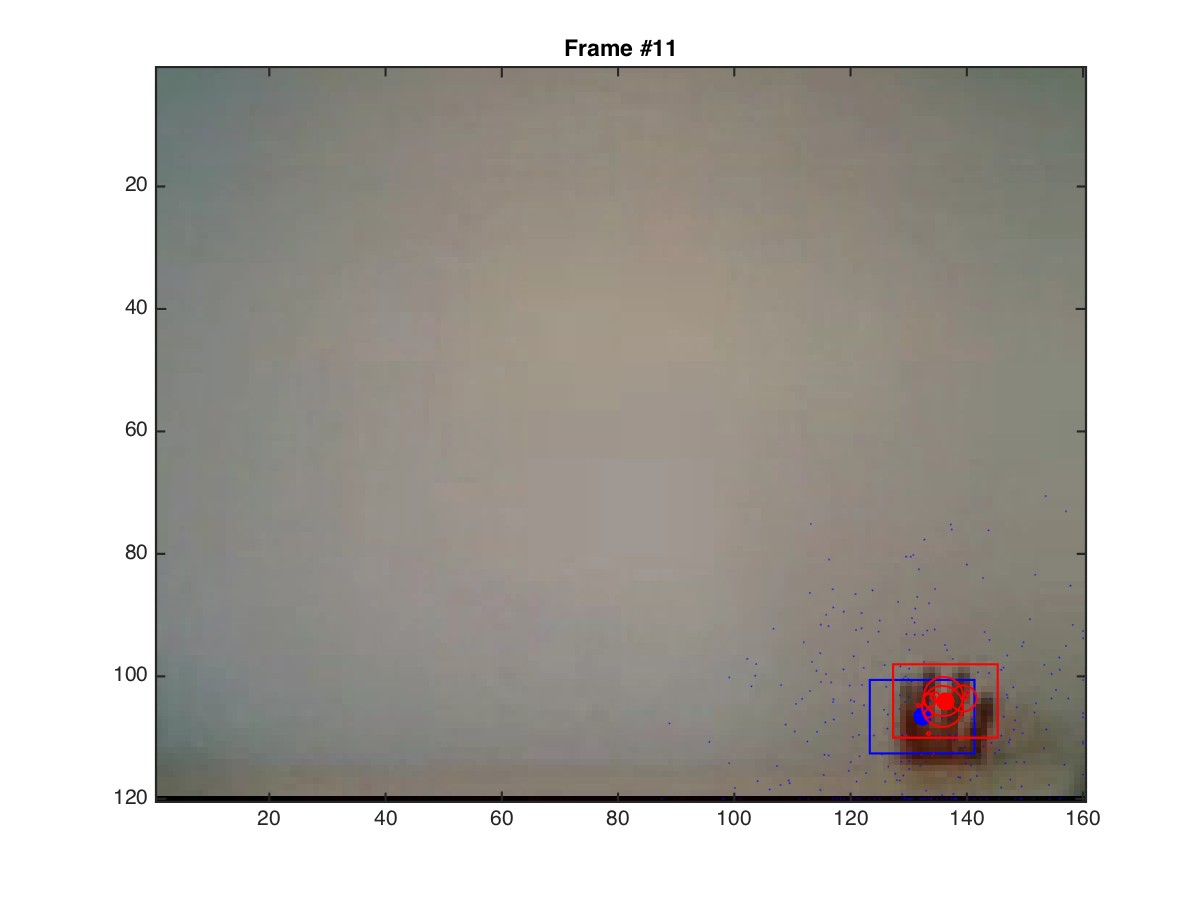
\includegraphics[width=1\linewidth]{images/video1_1}
    \end{subfigure}%
    \begin{subfigure}[b]{.25\textwidth}
        \centering
        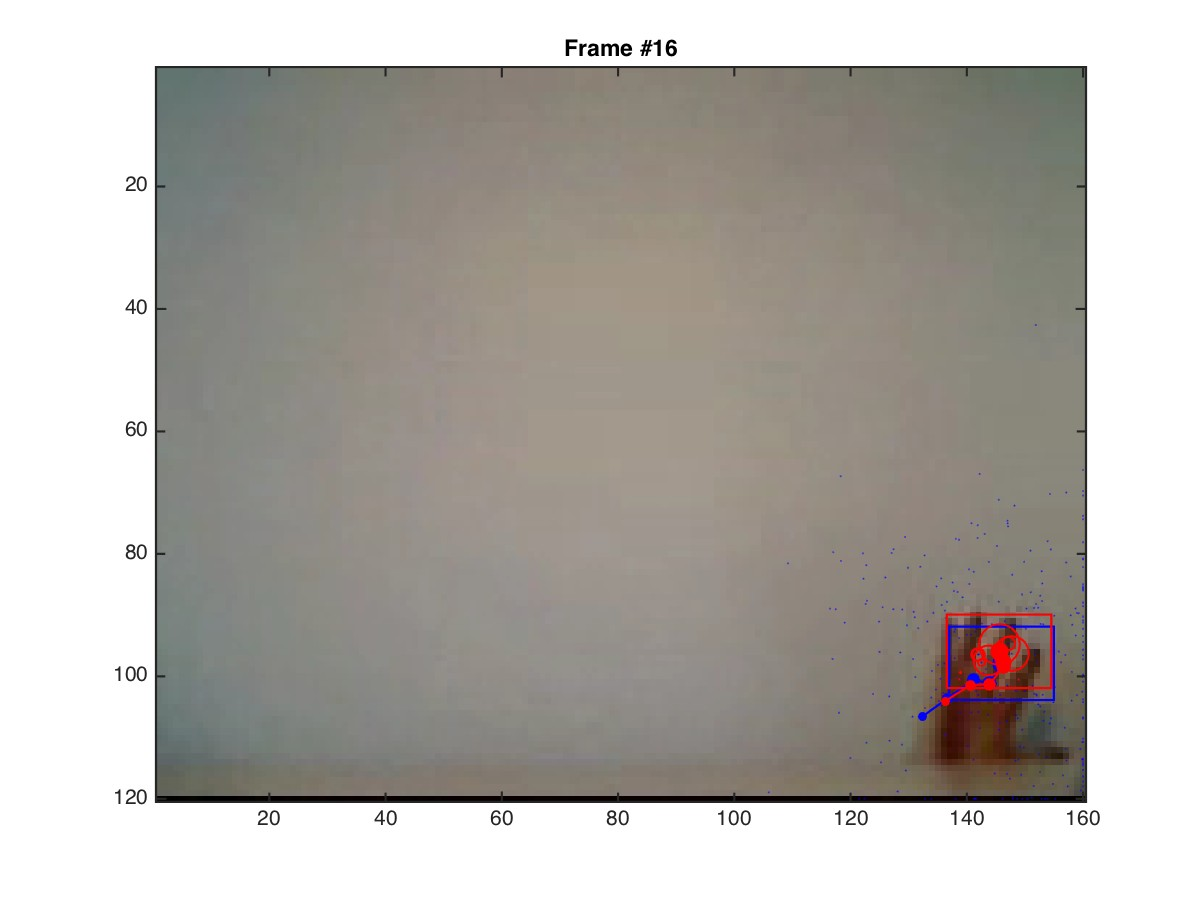
\includegraphics[width=1\linewidth]{images/video1_6}
    \end{subfigure}%
    \begin{subfigure}[b]{.25\textwidth}
        \centering
        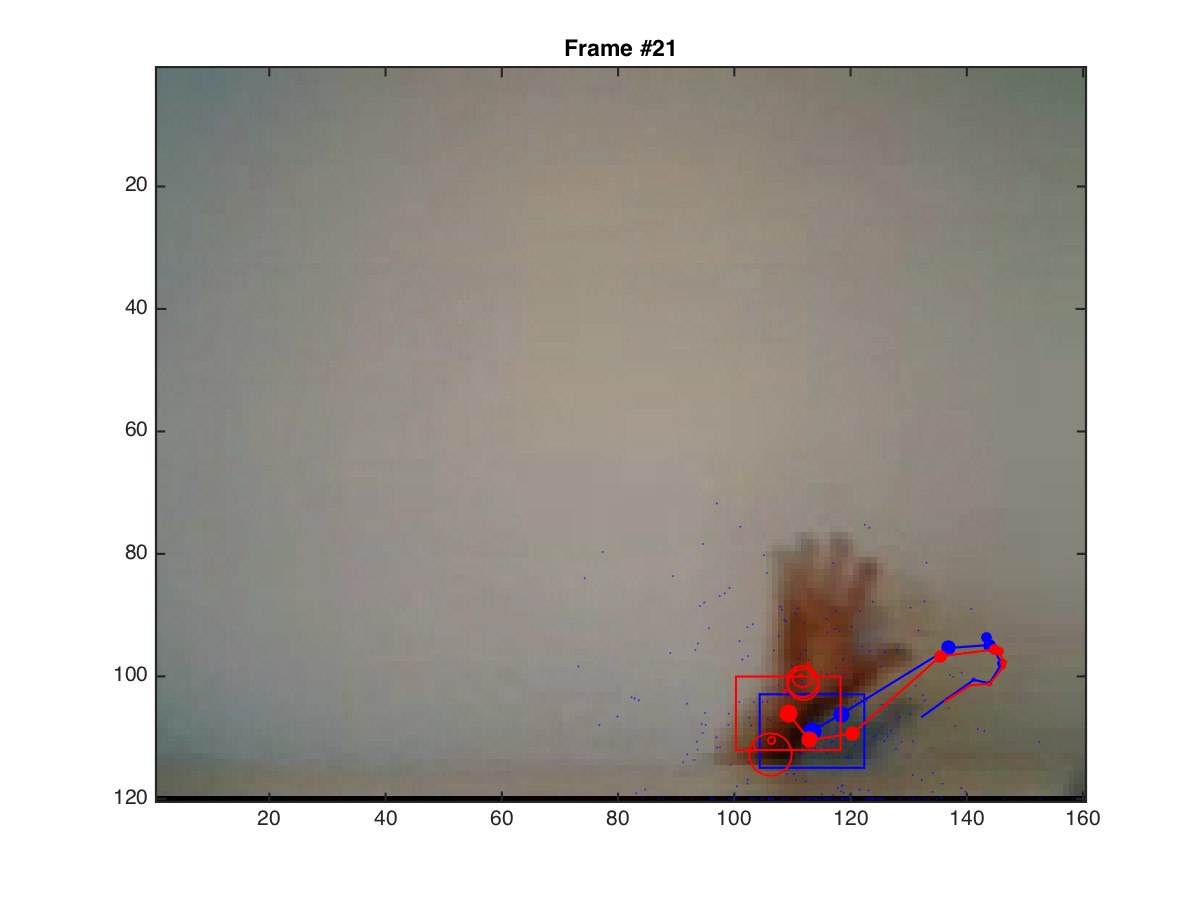
\includegraphics[width=1\linewidth]{images/video1_11}
    \end{subfigure}%
    \begin{subfigure}[b]{.25\textwidth}
        \centering
        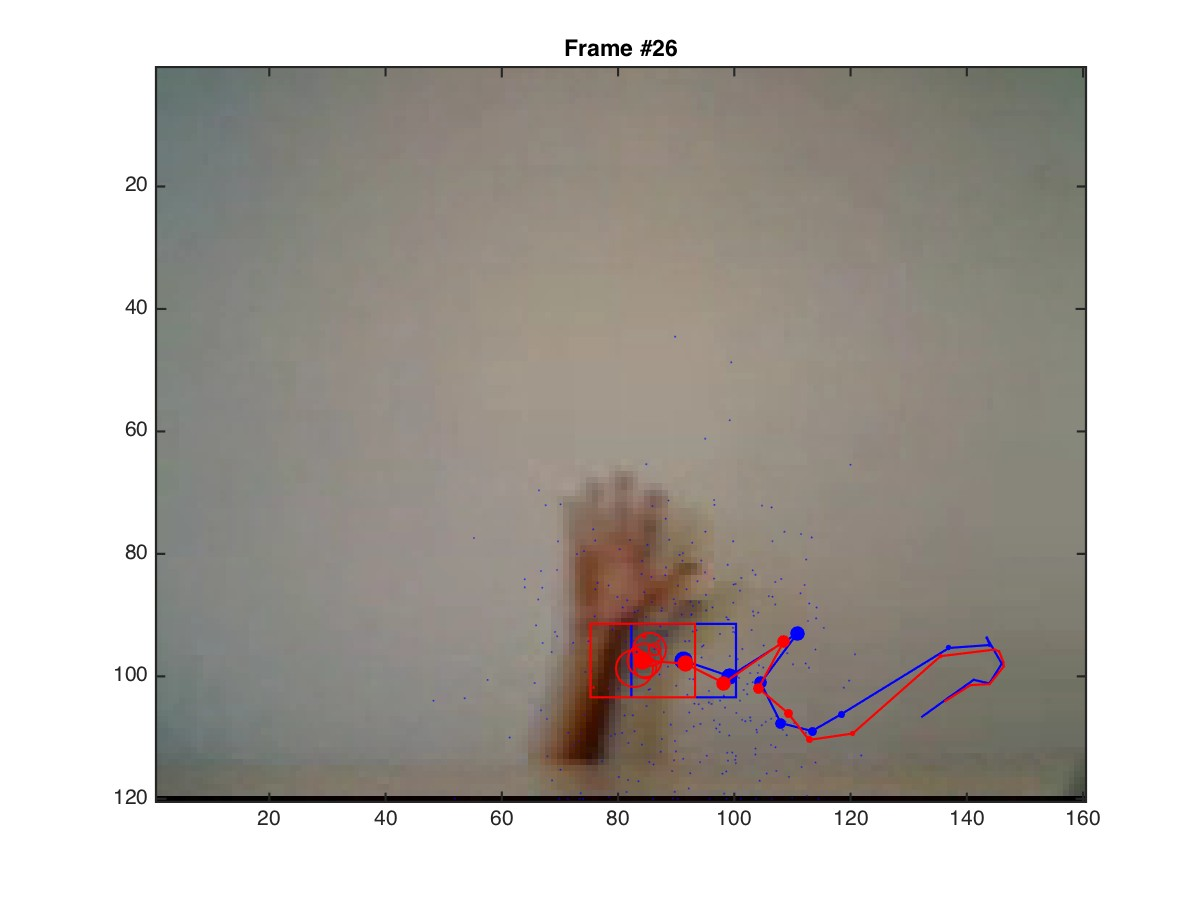
\includegraphics[width=1\linewidth]{images/video1_16}
    \end{subfigure}
    \begin{subfigure}[b]{.25\textwidth}
        \centering
        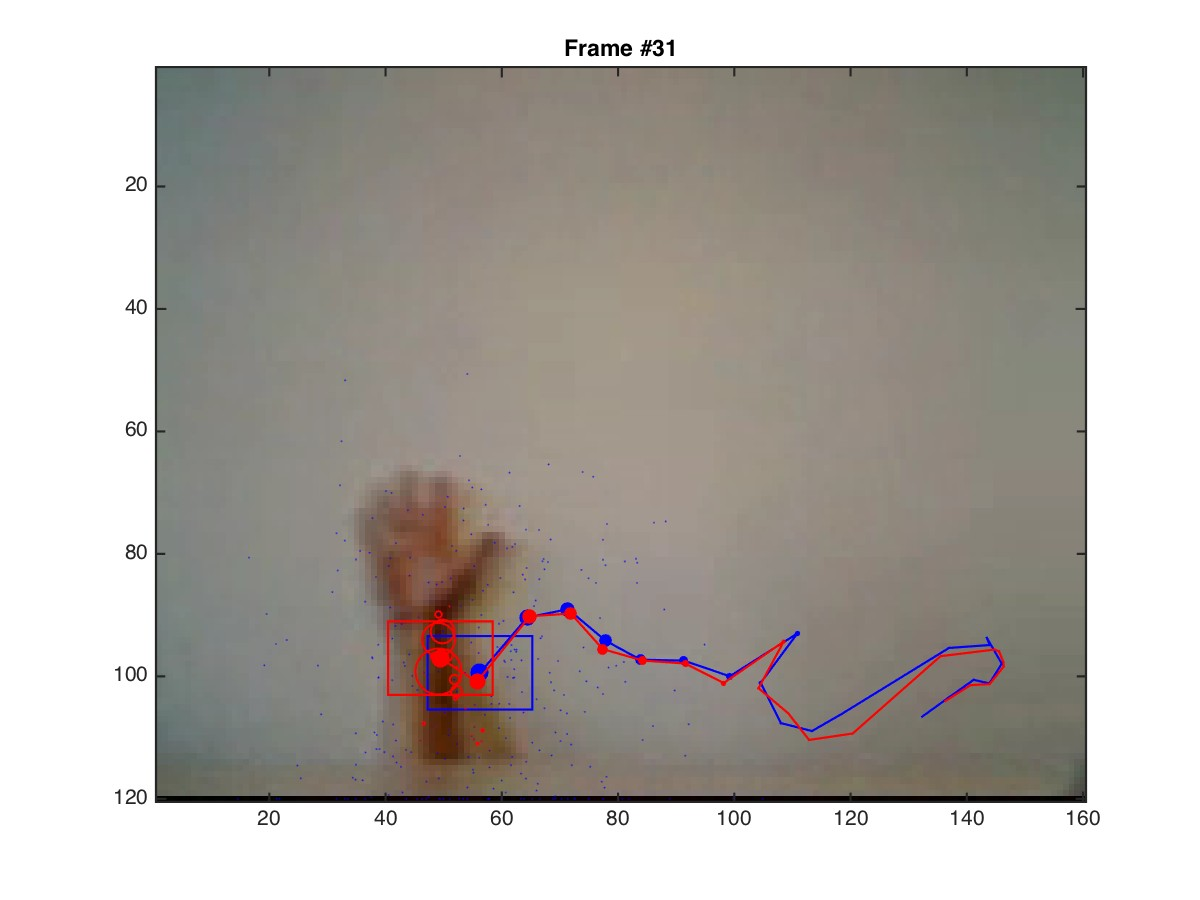
\includegraphics[width=1\linewidth]{images/video1_21}
    \end{subfigure}%
    \begin{subfigure}[b]{.25\textwidth}
        \centering
        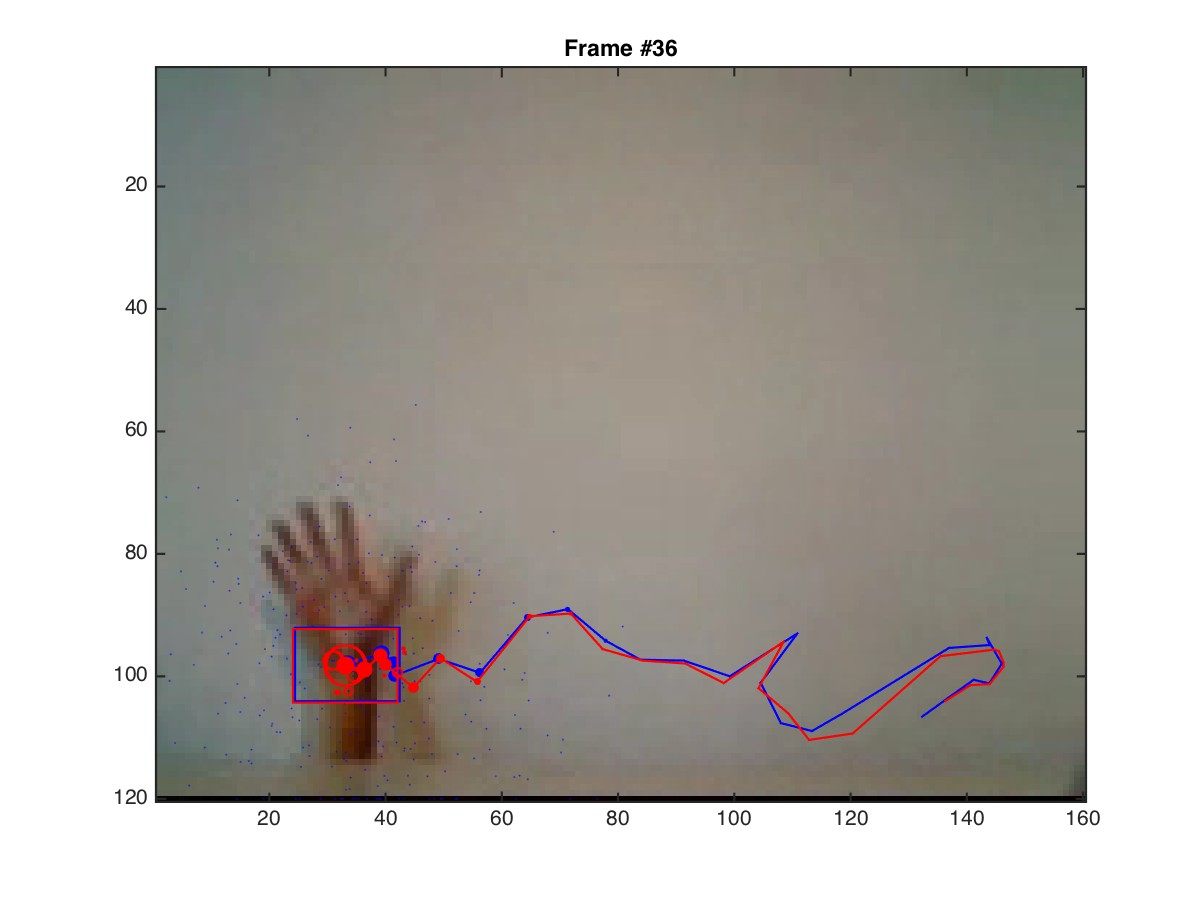
\includegraphics[width=1\linewidth]{images/video1_26}
    \end{subfigure}%
    \begin{subfigure}[b]{.25\textwidth}
        \centering
        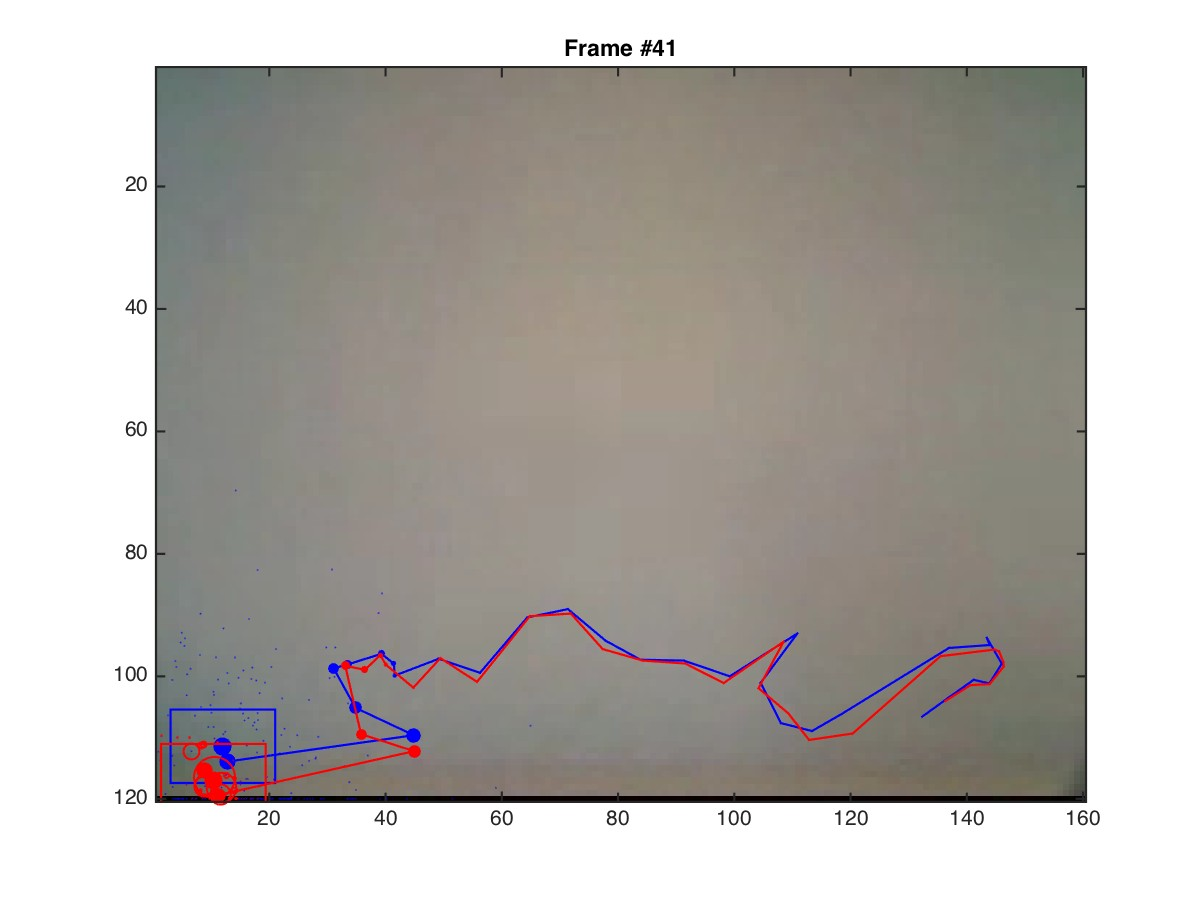
\includegraphics[width=1\linewidth]{images/video1_31}
    \end{subfigure}
    \caption{Tracking of the hand at the first video using the implemented Condensation Tracker}
    \label{fig:tracking_video1}
\end{figure}

\subsection*{\texttt{video2.wmv}}

First, with the default parameters, on Figure~\ref{fig:tracking_video1} there is the tracking for \texttt{vide2.wmv}. It can be seen how the tracker has been able to follow the object even whit an occlusion.

\begin{figure}[h]
    \centering
    \begin{subfigure}[b]{.25\textwidth}
        \centering
        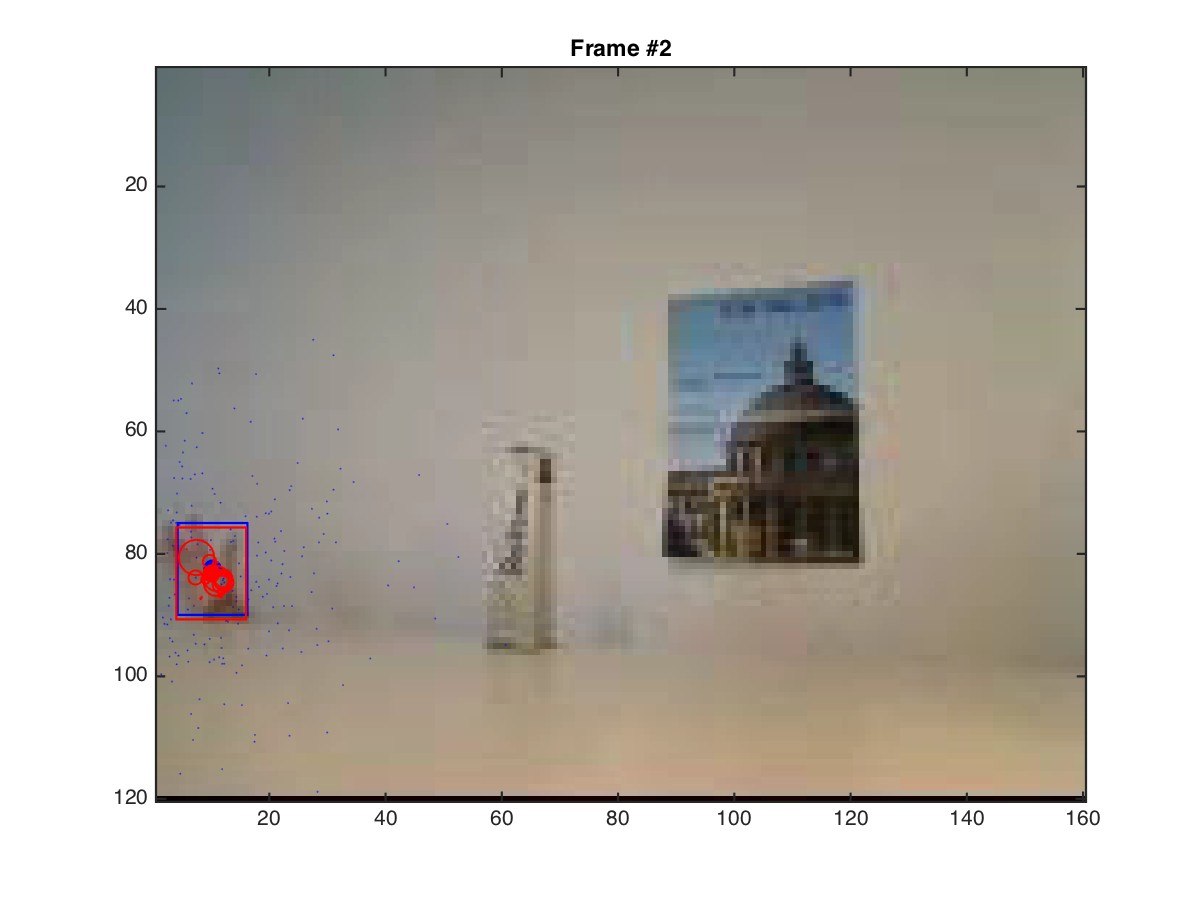
\includegraphics[width=1\linewidth]{images/video2__1}
    \end{subfigure}%
    \begin{subfigure}[b]{.25\textwidth}
        \centering
        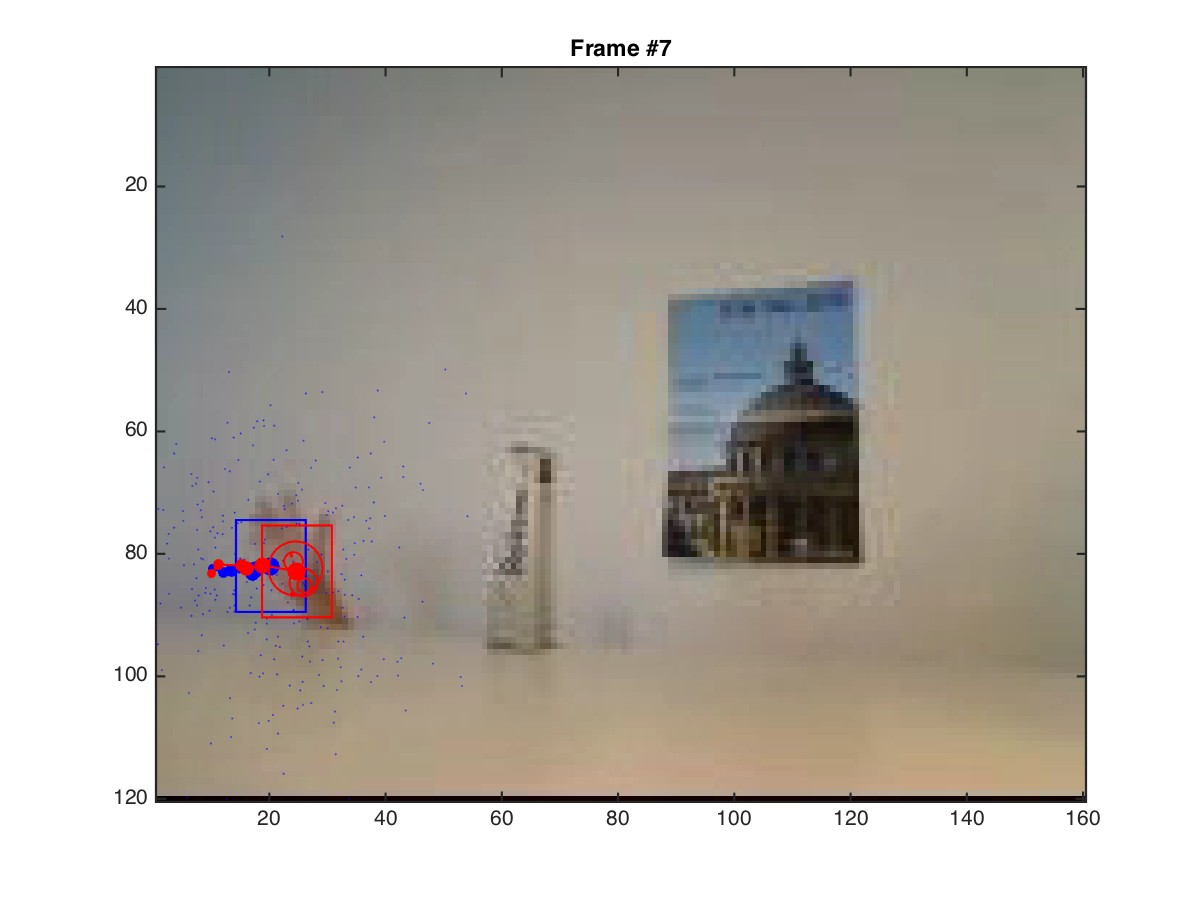
\includegraphics[width=1\linewidth]{images/video2__6}
    \end{subfigure}%
    \begin{subfigure}[b]{.25\textwidth}
        \centering
        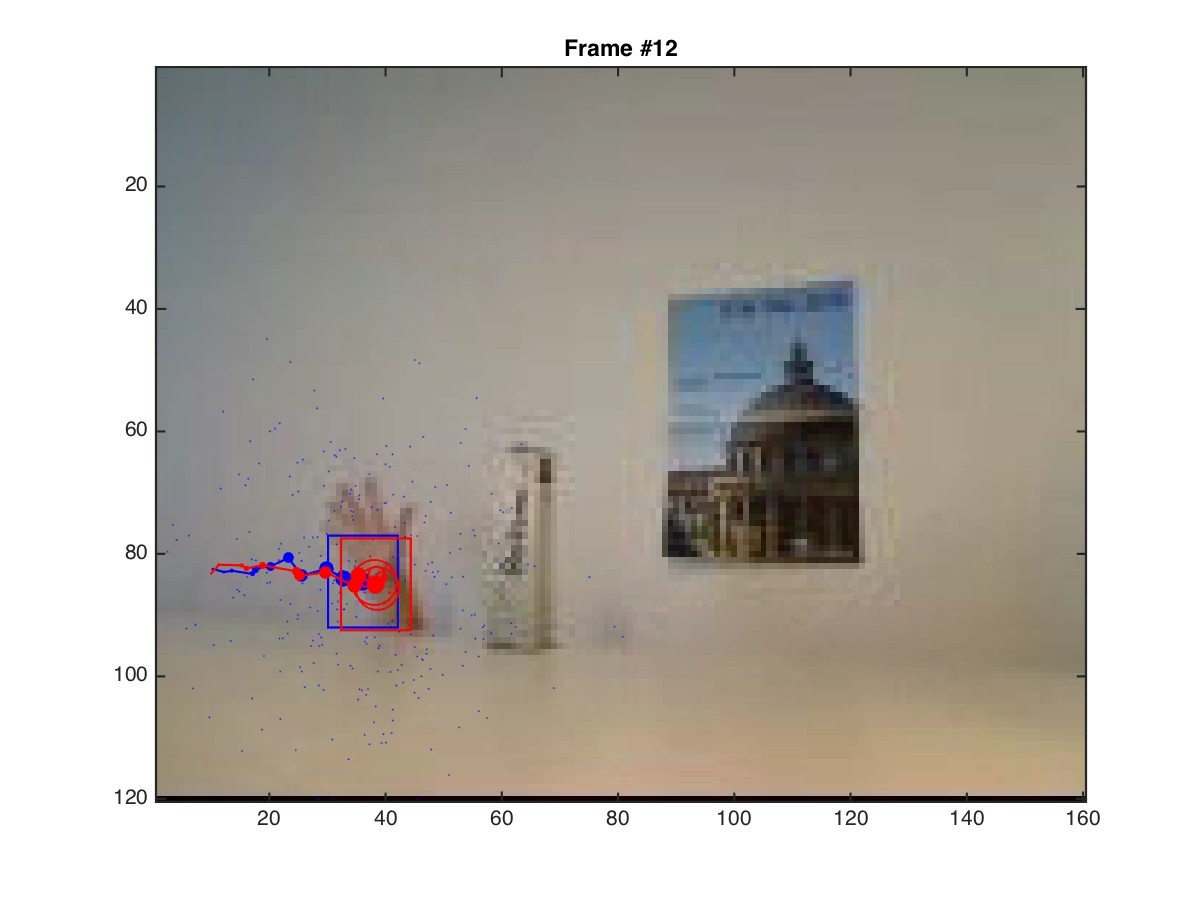
\includegraphics[width=1\linewidth]{images/video2__11}
    \end{subfigure}%
    \begin{subfigure}[b]{.25\textwidth}
        \centering
        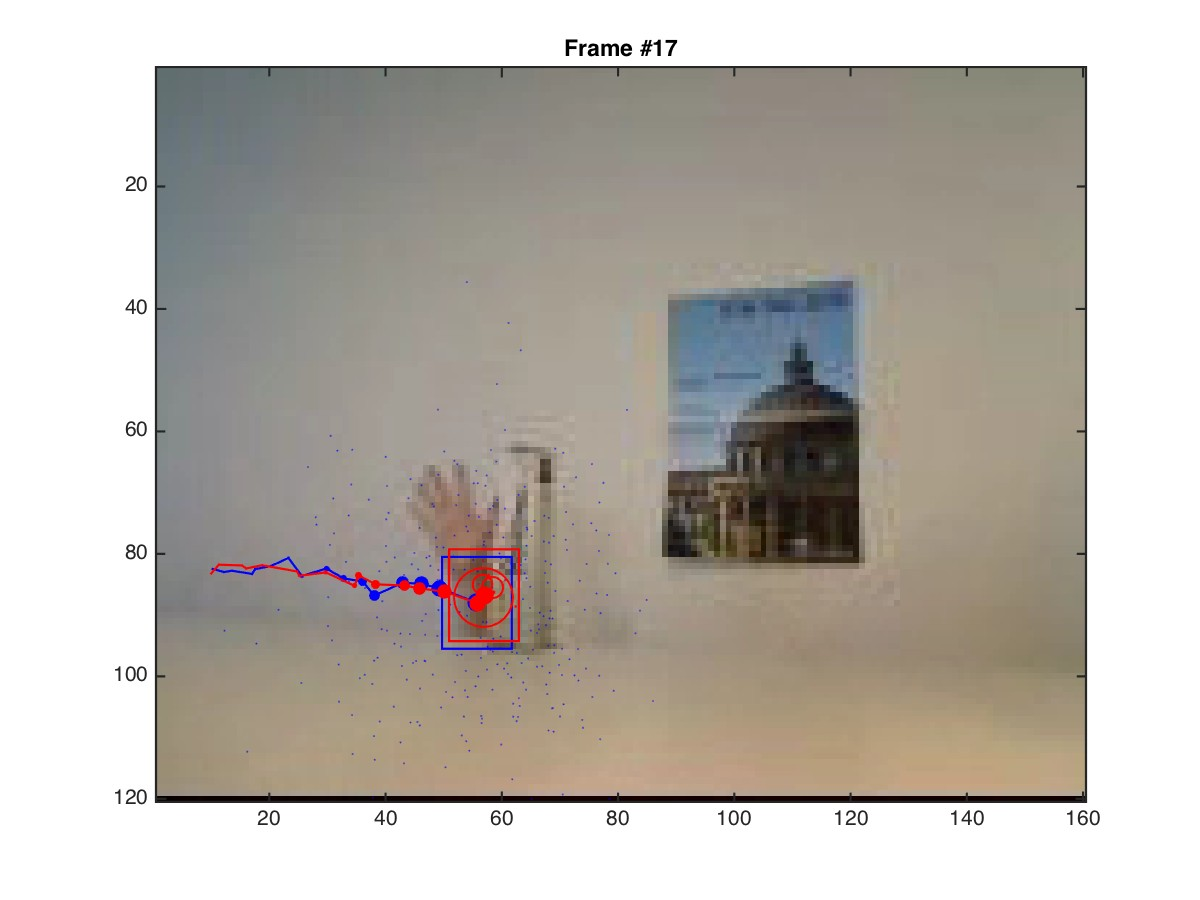
\includegraphics[width=1\linewidth]{images/video2__16}
    \end{subfigure}
    \begin{subfigure}[b]{.25\textwidth}
        \centering
        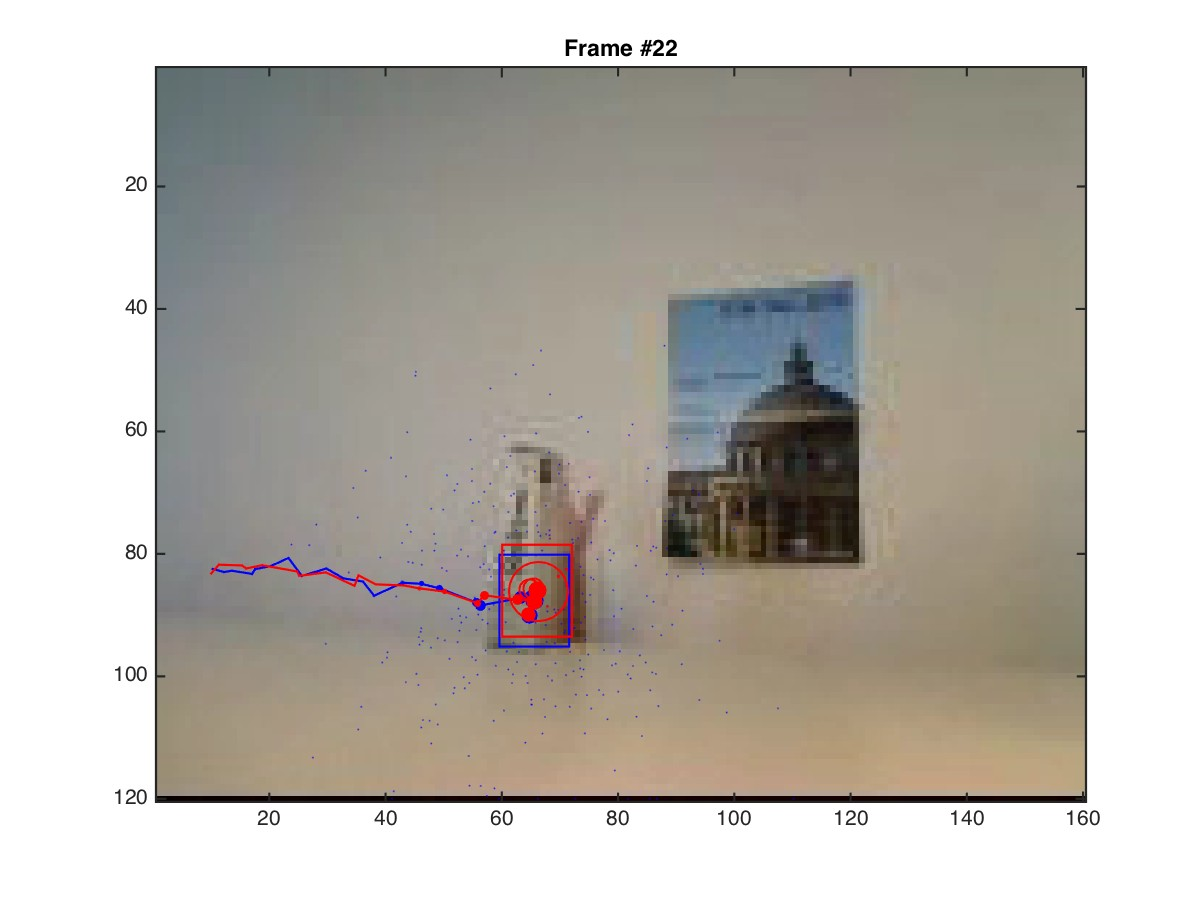
\includegraphics[width=1\linewidth]{images/video2__21}
    \end{subfigure}%
    \begin{subfigure}[b]{.25\textwidth}
        \centering
        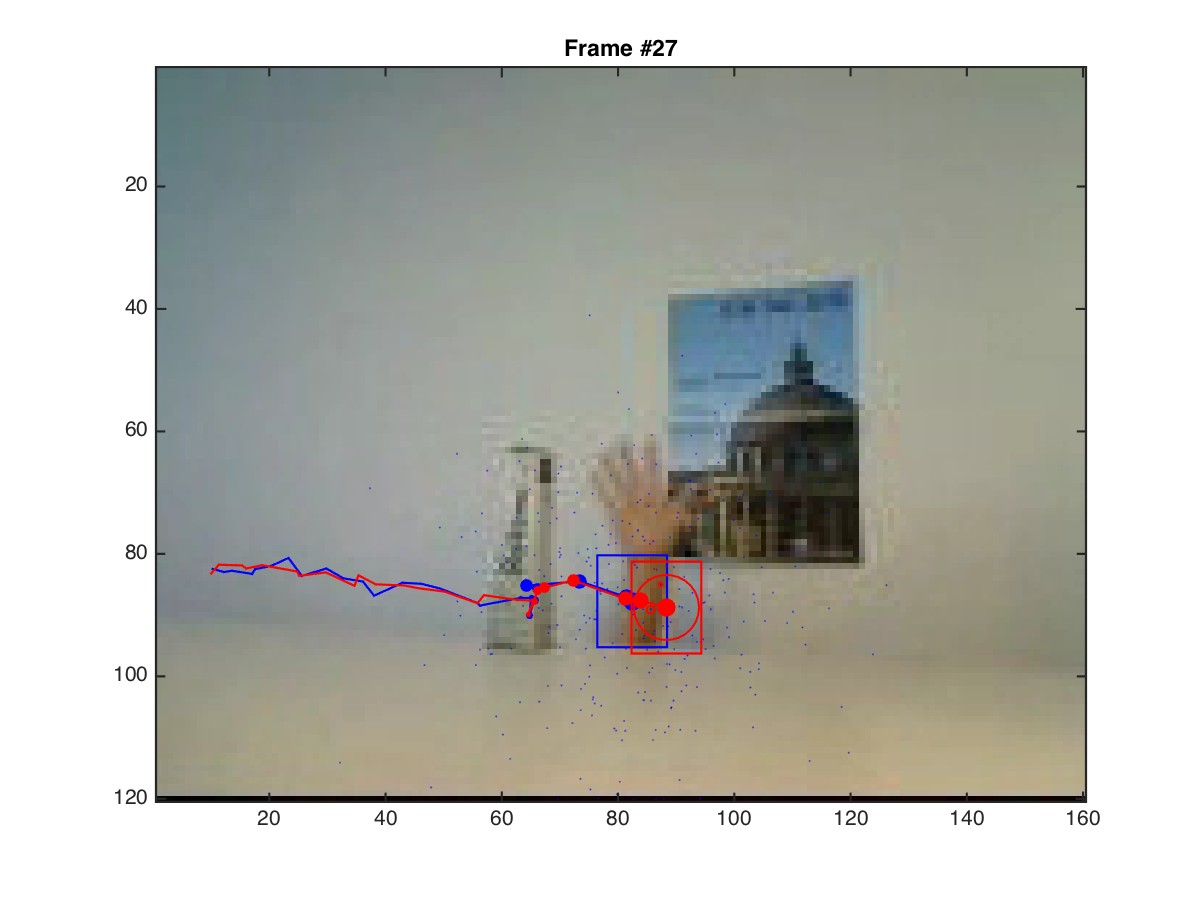
\includegraphics[width=1\linewidth]{images/video2__26}
    \end{subfigure}%
    \begin{subfigure}[b]{.25\textwidth}
        \centering
        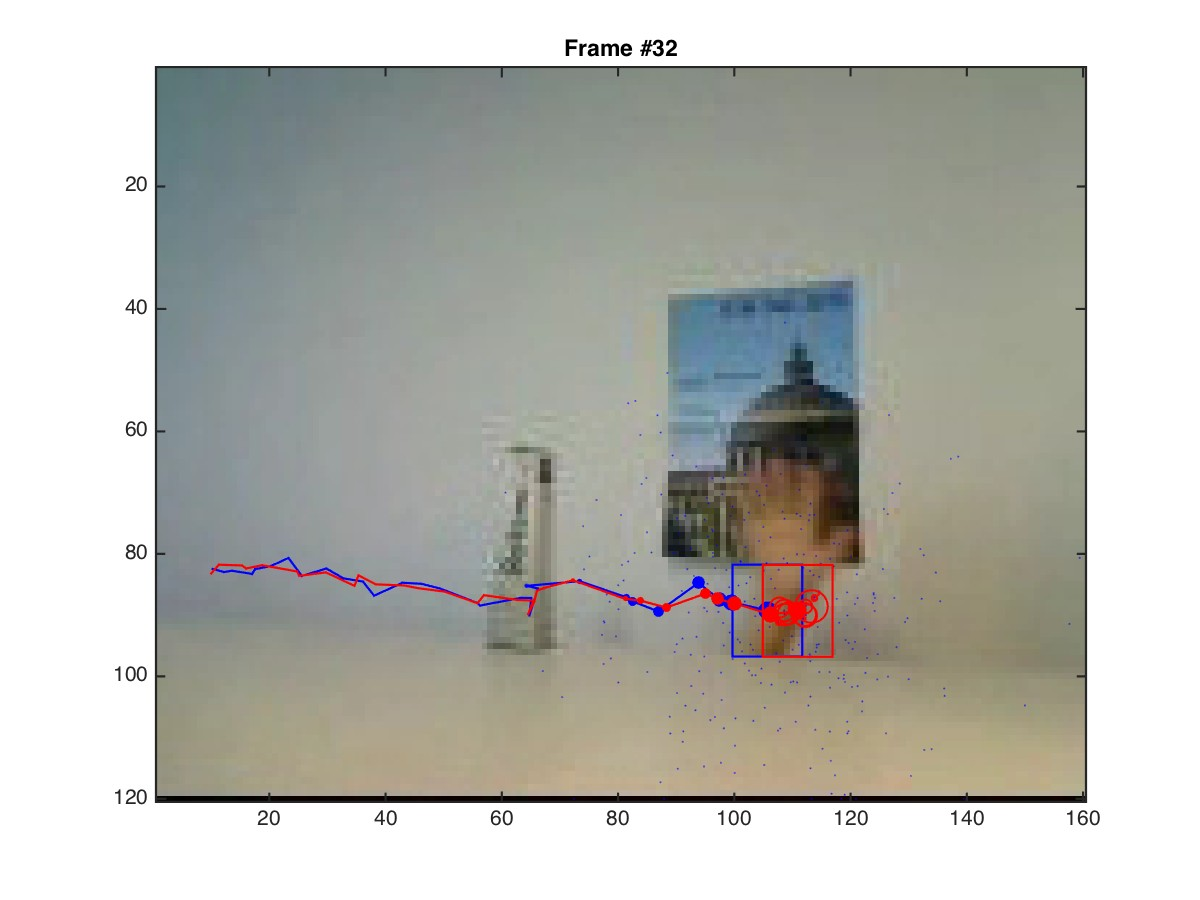
\includegraphics[width=1\linewidth]{images/video2__31}
    \end{subfigure}%
    \begin{subfigure}[b]{.25\textwidth}
        \centering
        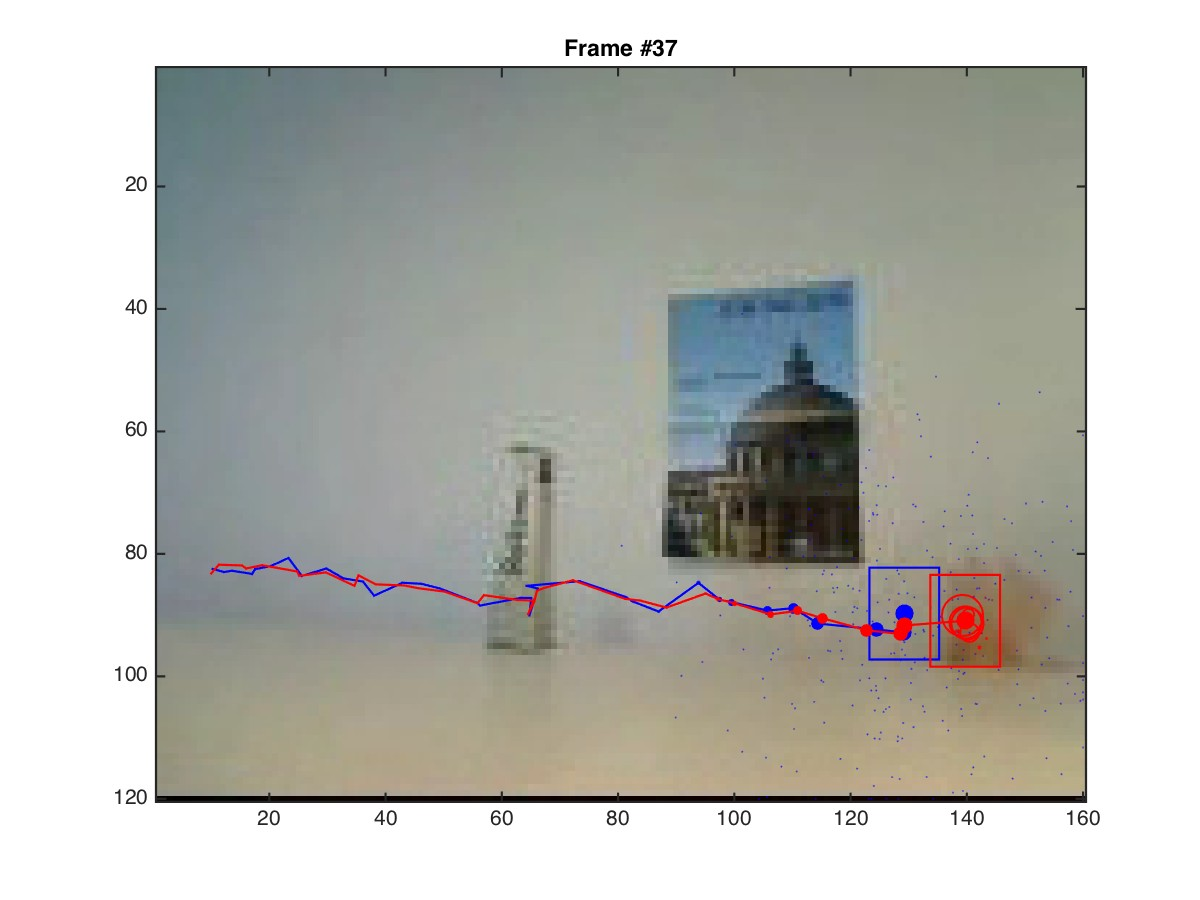
\includegraphics[width=1\linewidth]{images/video2__36}
    \end{subfigure}
    \caption{Tracking of the hand at \texttt{video2.wmv} using the implemented Condensation Tracker}
    \label{fig:tracking_video2}
\end{figure}

\subsubsection*{Effect of the model}

In order to study the performance of the tracker depending on its parameters, first, the constant velocity model is tested.
The tracking is on Figure~\ref{fig:tracking_video2_model} where it can be seen how, as the initial velocity was set wit $v_0 = [ 1, 10 ]^T$, the prior probability distribution tent to predict in a lower position in the vertical axis.
But thanks to the observations, and the enough dispersion of the particles, the posterior probability perfectly tracks the object even when this is occluded.

\begin{figure}[h]
    \centering
    \begin{subfigure}[b]{.25\textwidth}
        \centering
        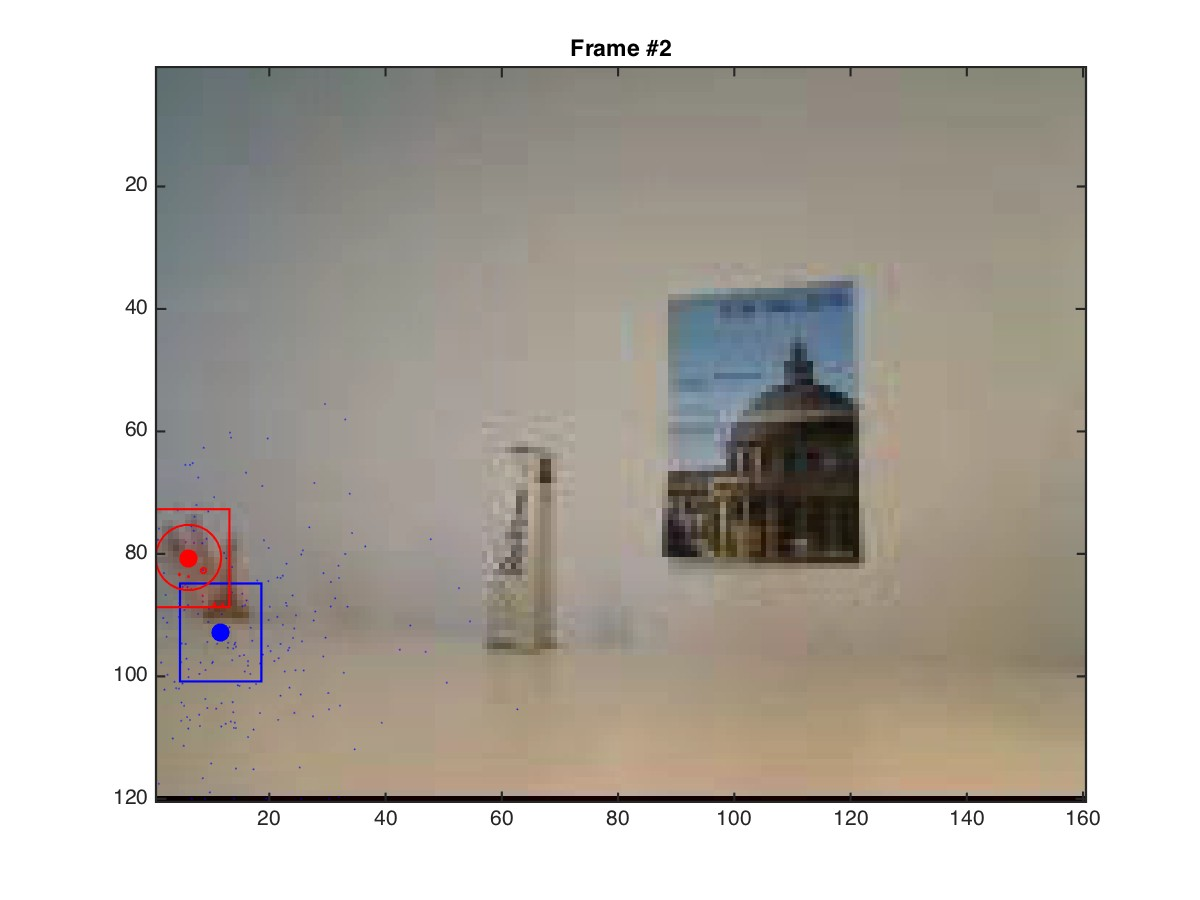
\includegraphics[width=1\linewidth]{images/video2_model_1}
    \end{subfigure}%
    \begin{subfigure}[b]{.25\textwidth}
        \centering
        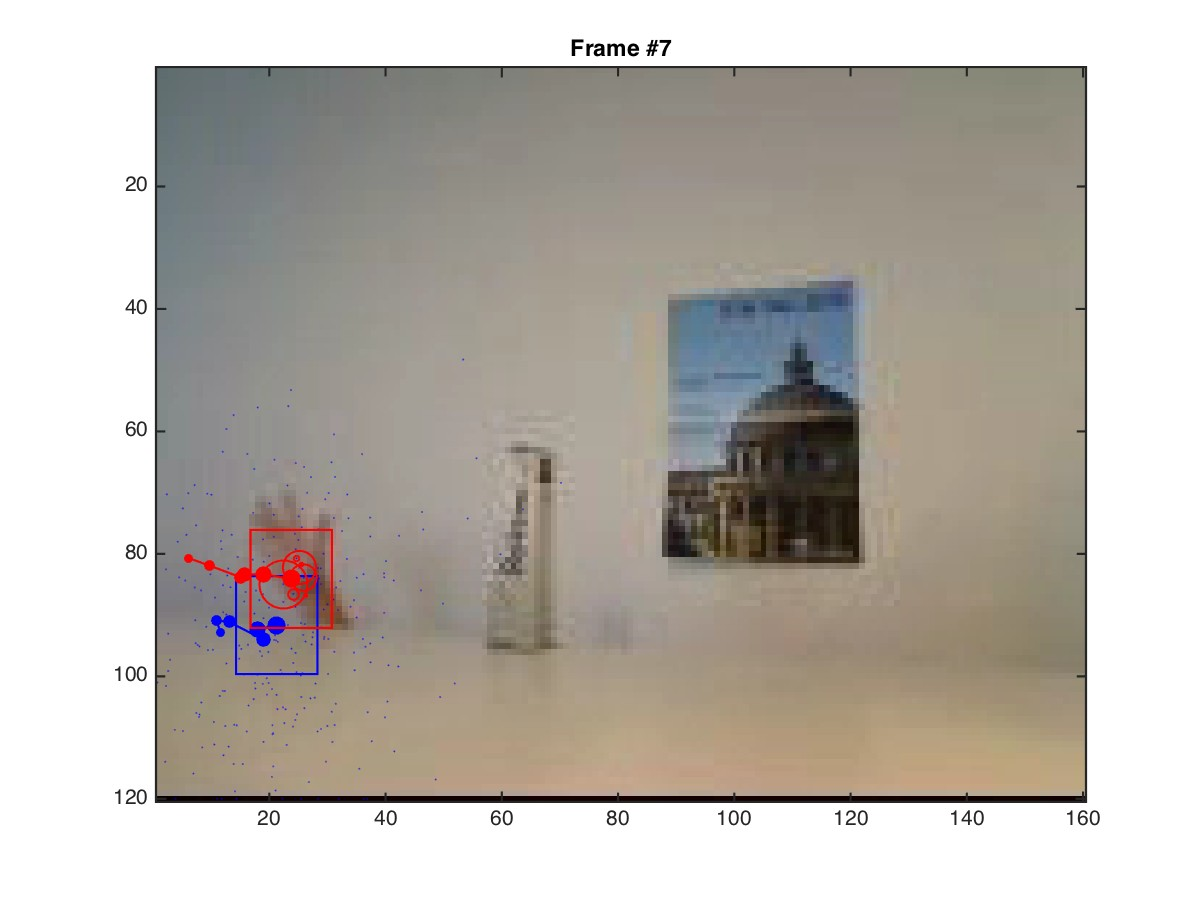
\includegraphics[width=1\linewidth]{images/video2_model_6}
    \end{subfigure}%
    \begin{subfigure}[b]{.25\textwidth}
        \centering
        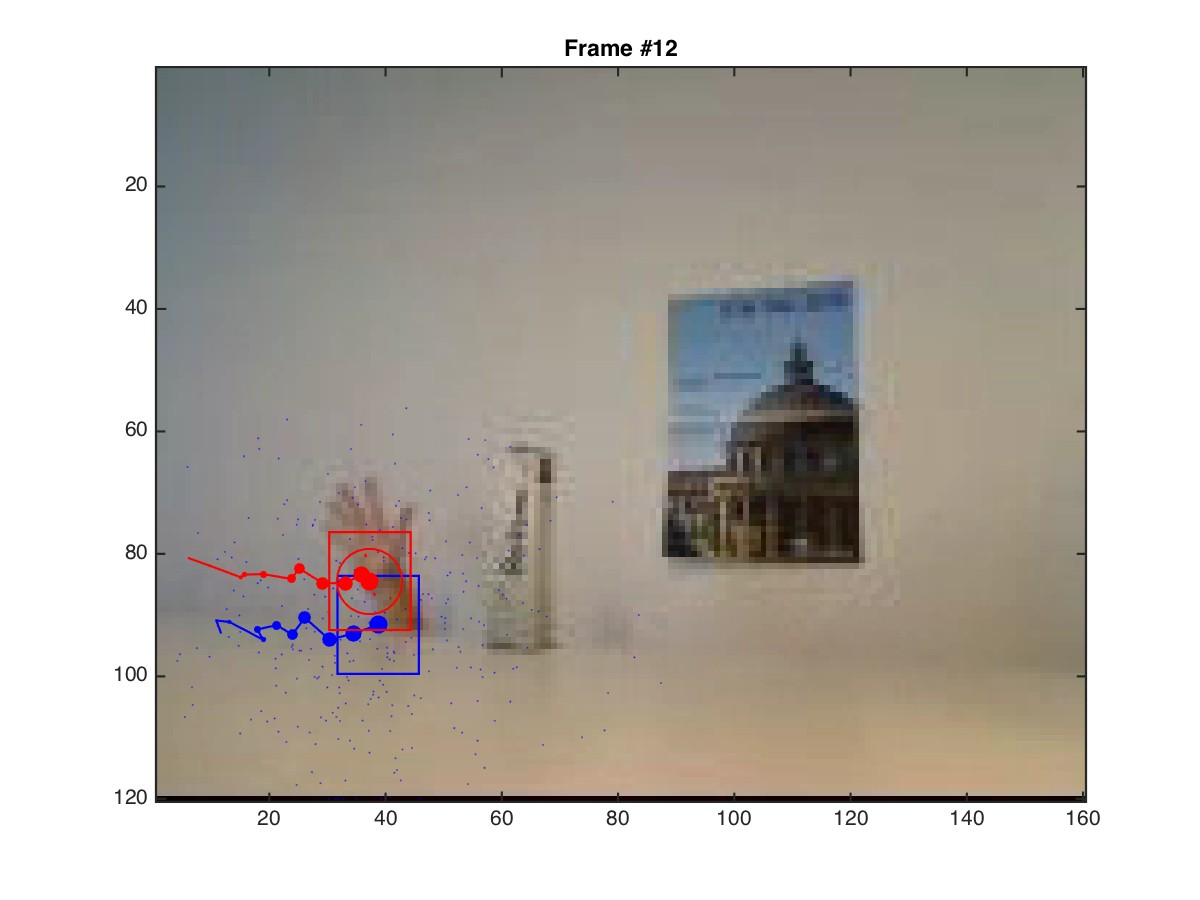
\includegraphics[width=1\linewidth]{images/video2_model_11}
    \end{subfigure}%
    \begin{subfigure}[b]{.25\textwidth}
        \centering
        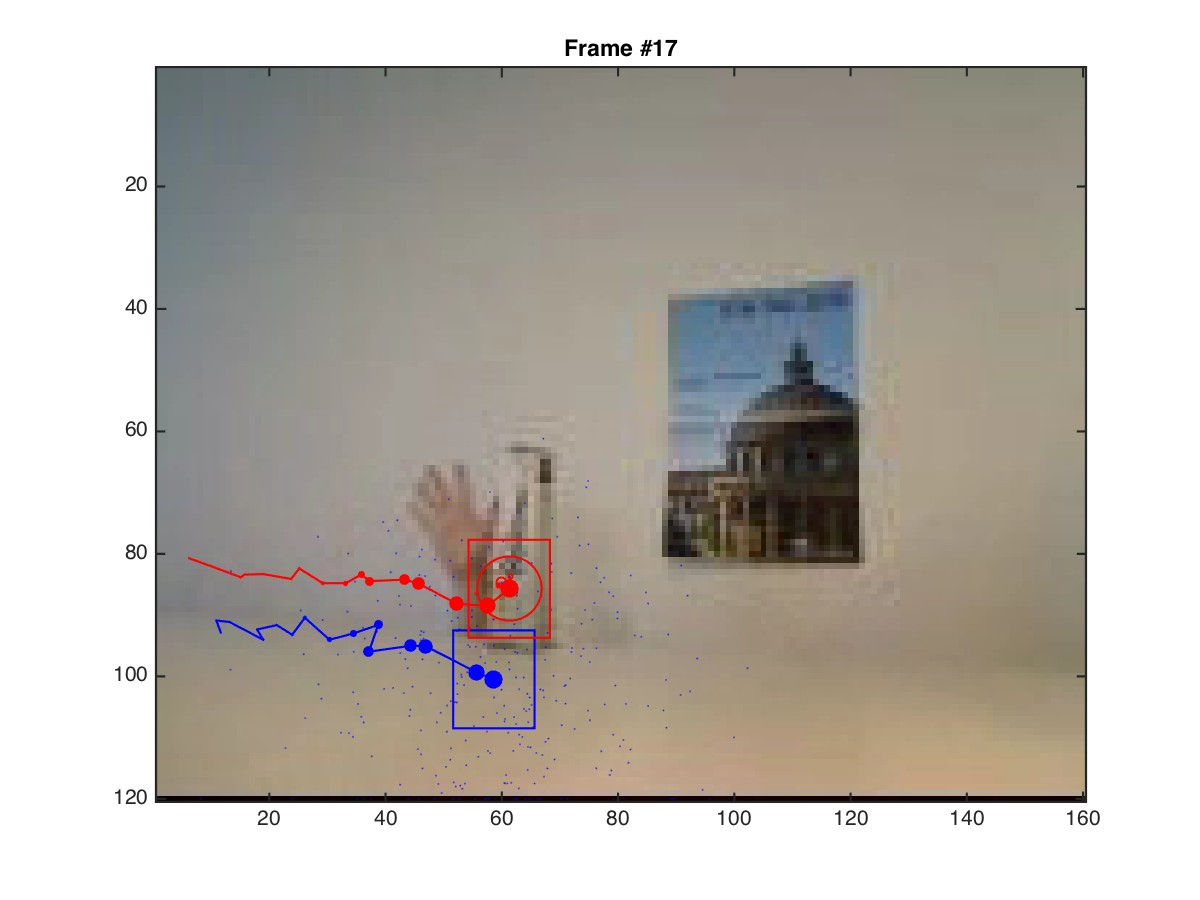
\includegraphics[width=1\linewidth]{images/video2_model_16}
    \end{subfigure}
    \begin{subfigure}[b]{.25\textwidth}
        \centering
        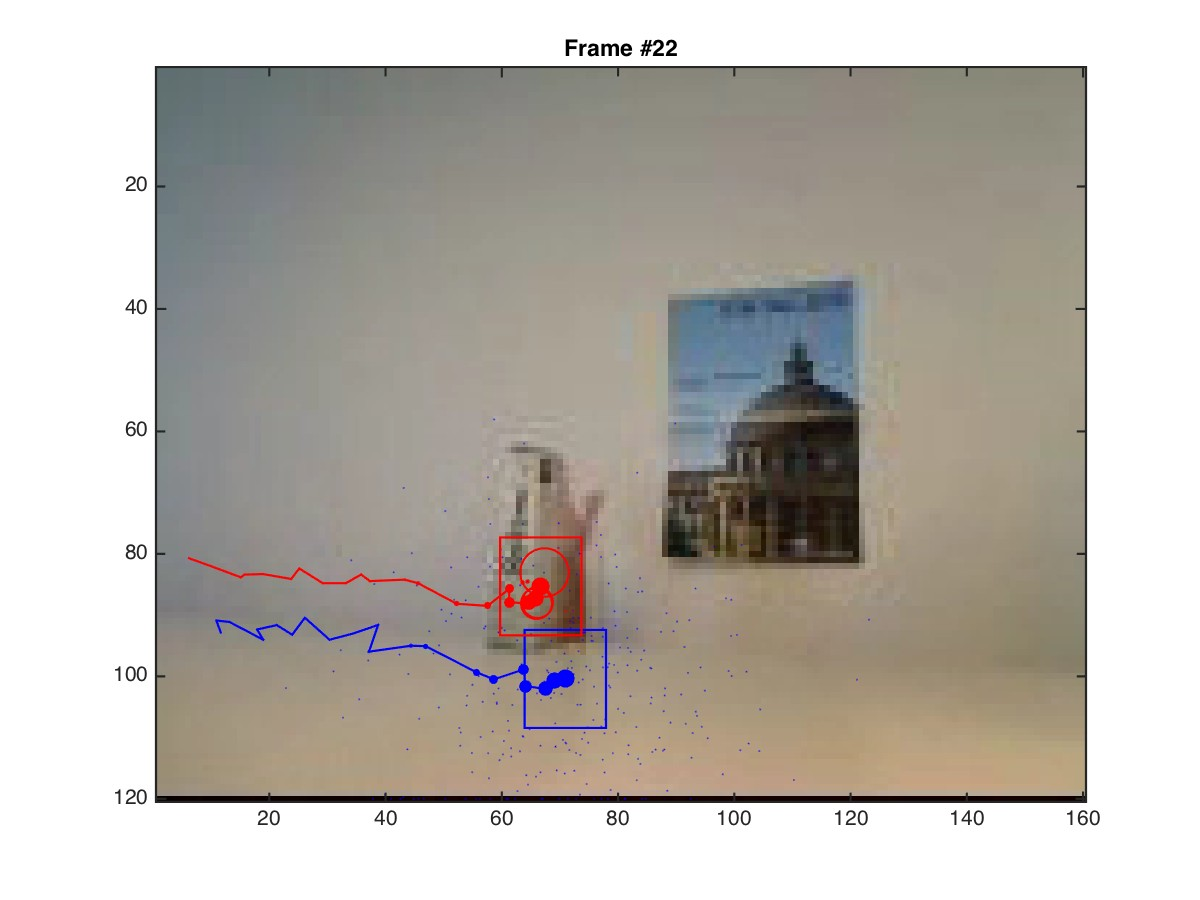
\includegraphics[width=1\linewidth]{images/video2_model_21}
    \end{subfigure}%
    \begin{subfigure}[b]{.25\textwidth}
        \centering
        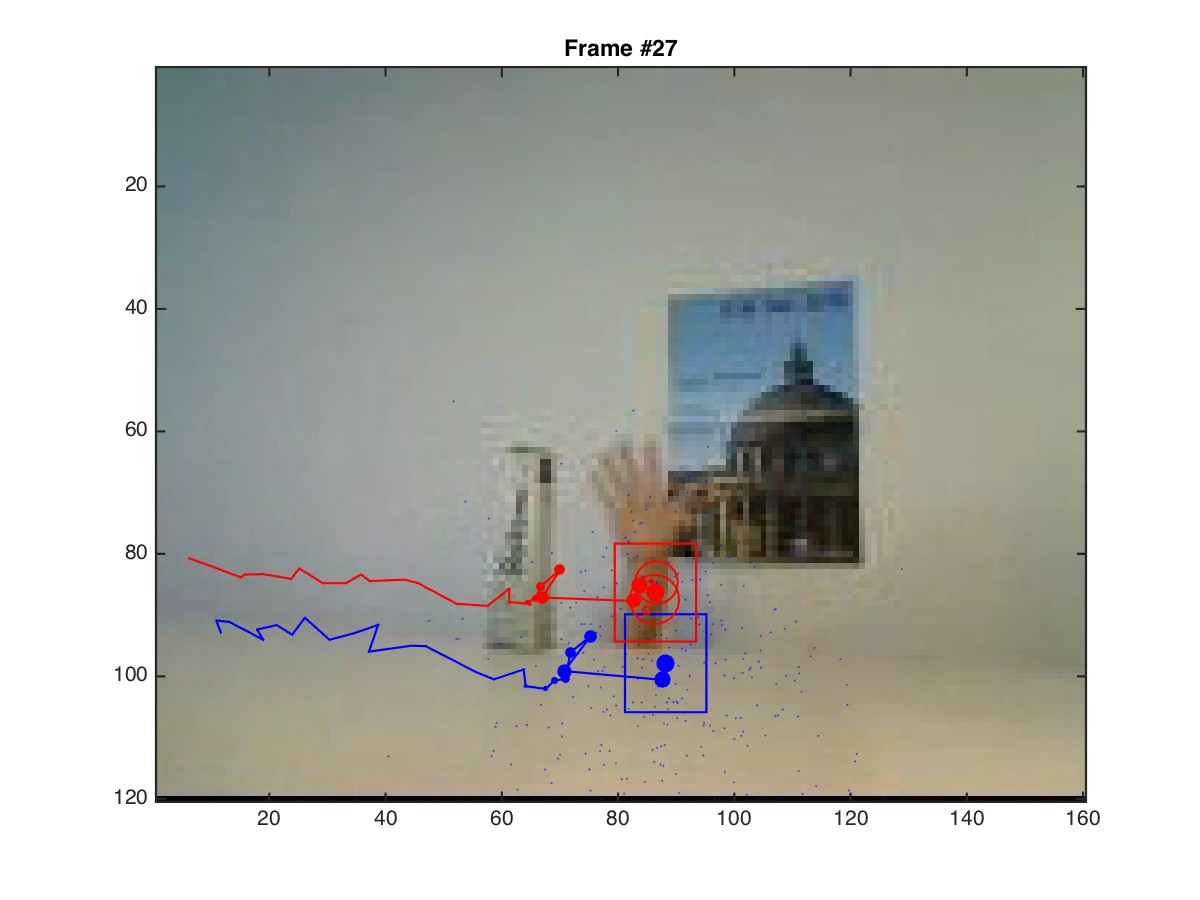
\includegraphics[width=1\linewidth]{images/video2_model_26}
    \end{subfigure}%
    \begin{subfigure}[b]{.25\textwidth}
        \centering
        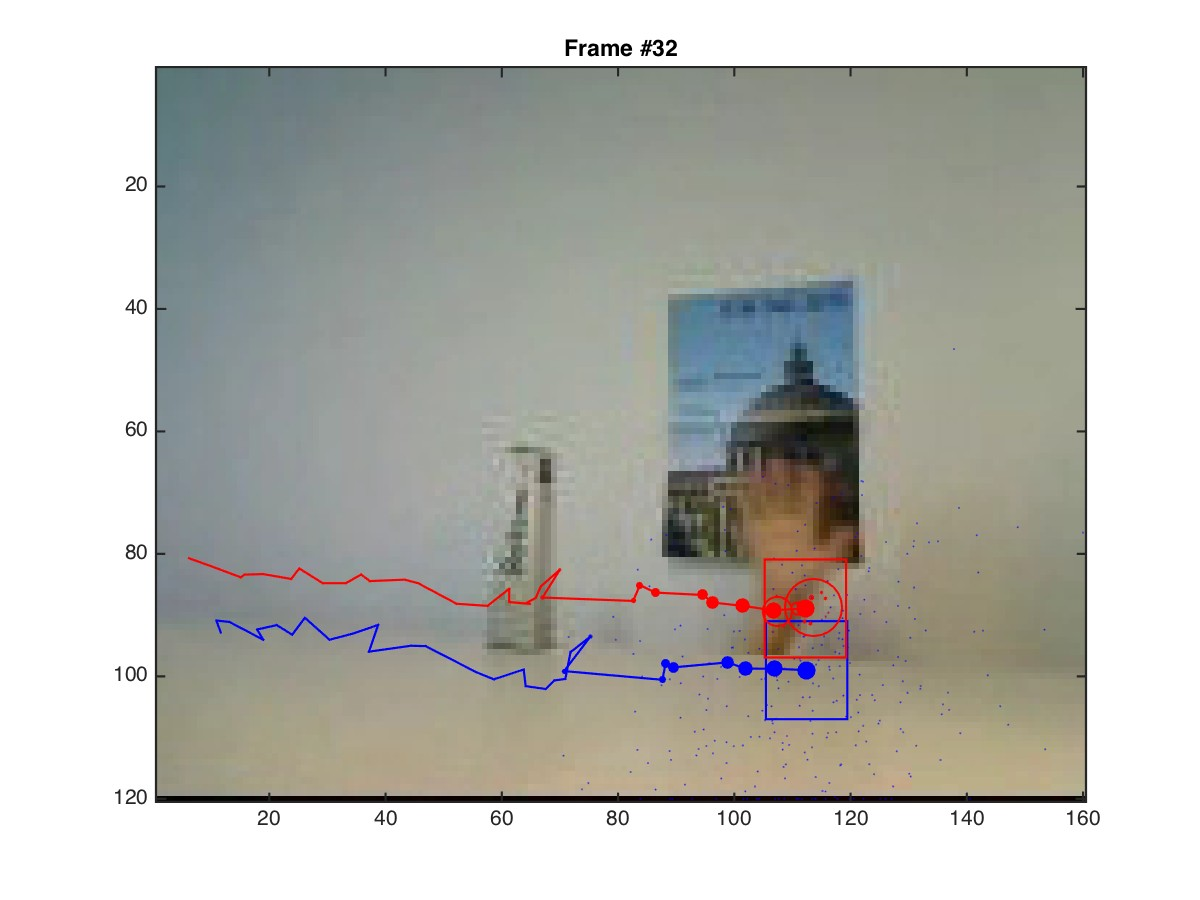
\includegraphics[width=1\linewidth]{images/video2_model_31}
    \end{subfigure}%
    \begin{subfigure}[b]{.25\textwidth}
        \centering
        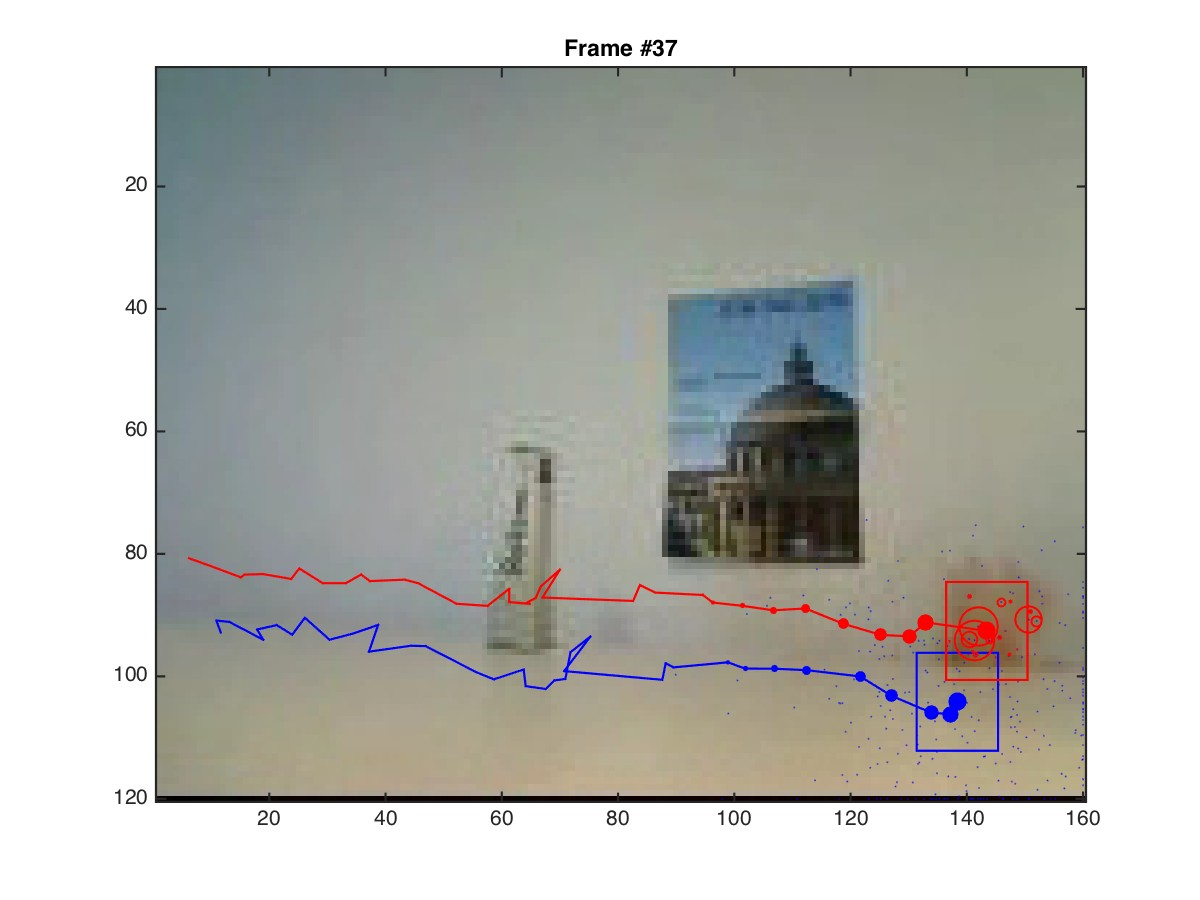
\includegraphics[width=1\linewidth]{images/video2_model_36}
    \end{subfigure}
    \caption{Tracking for \texttt{video2.wmv} with the constant velocity model.}
    \label{fig:tracking_video2_model}
\end{figure}

\subsubsection*{Effect of the system noise}

To study the effect of the system noise, with the system that models the constant position and the rest of default parameters, the $\sigma_{position}$ has been set to high value and into a lower one to observe the differences in the tracking.

For a highly noise system, with $\sigma_{position} = 50$, the tracking is represented in Figure~\ref{fig:tracking_video2_noise_high} where it can be seen how the particles at each step spread along the image, leading to a prediction not very spatially precise as not many particles actually cover the object to track.
This makes the tracking very imprecise along the movement. It could be solved adding more particles, but this will increase substantially the computations cost.

On the other hand, using $\sigma_{position} = 5$, the tracking is more smooth as all the particles concentrate around the previous position as it can be seen in Figure~\ref{fig:tracking_video2_noise_low}.

\begin{figure}[h]
    \centering
    \begin{subfigure}[b]{.25\textwidth}
        \centering
        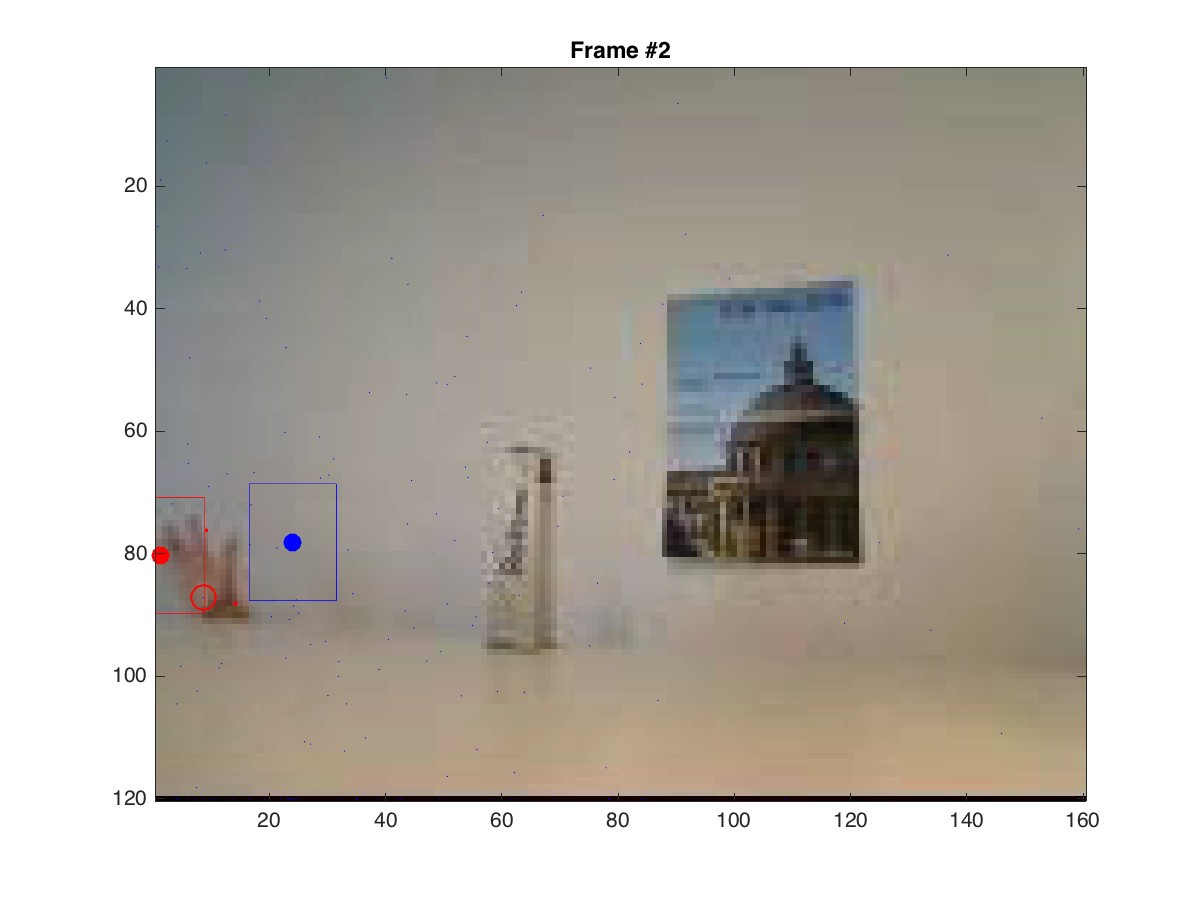
\includegraphics[width=1\linewidth]{images/video2_noise_high_1}
    \end{subfigure}%
    \begin{subfigure}[b]{.25\textwidth}
        \centering
        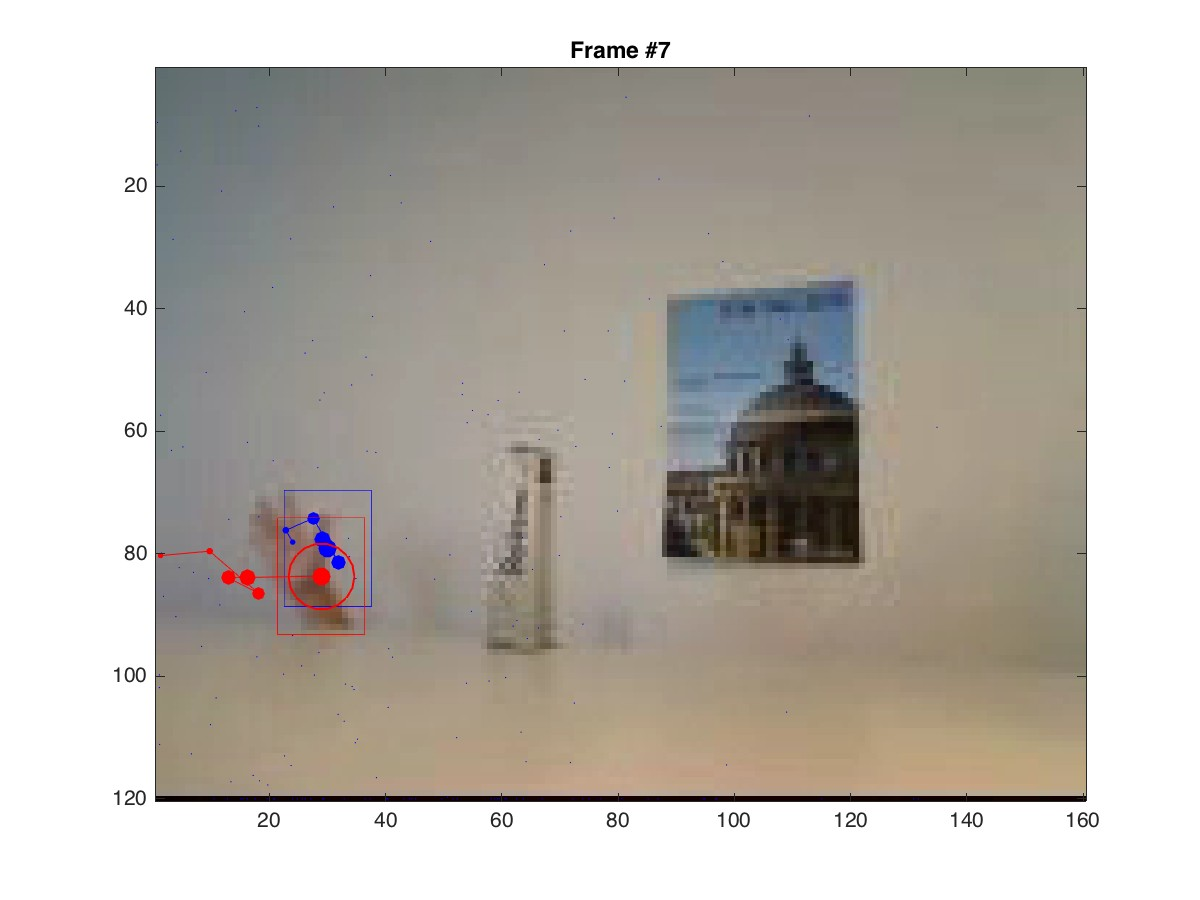
\includegraphics[width=1\linewidth]{images/video2_noise_high_6}
    \end{subfigure}%
    \begin{subfigure}[b]{.25\textwidth}
        \centering
        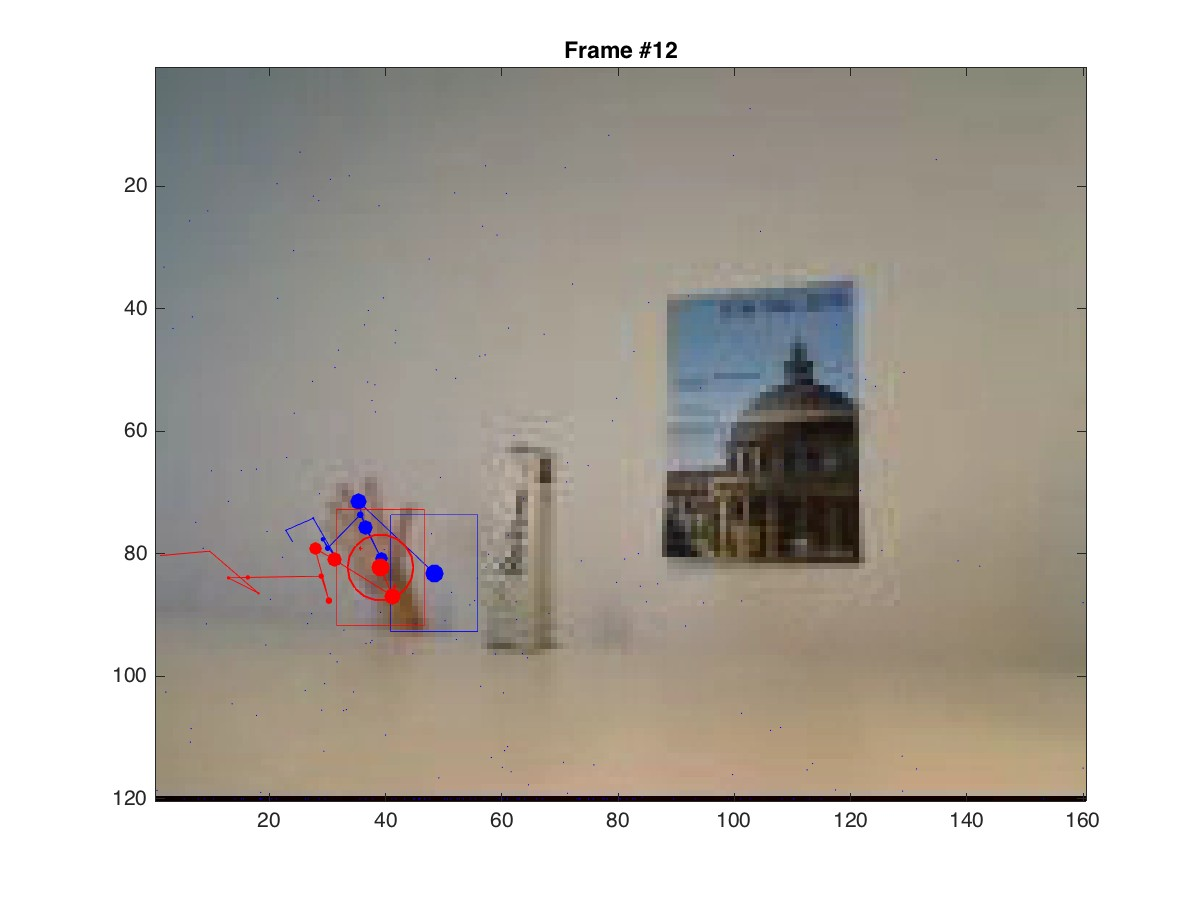
\includegraphics[width=1\linewidth]{images/video2_noise_high_11}
    \end{subfigure}%
    \begin{subfigure}[b]{.25\textwidth}
        \centering
        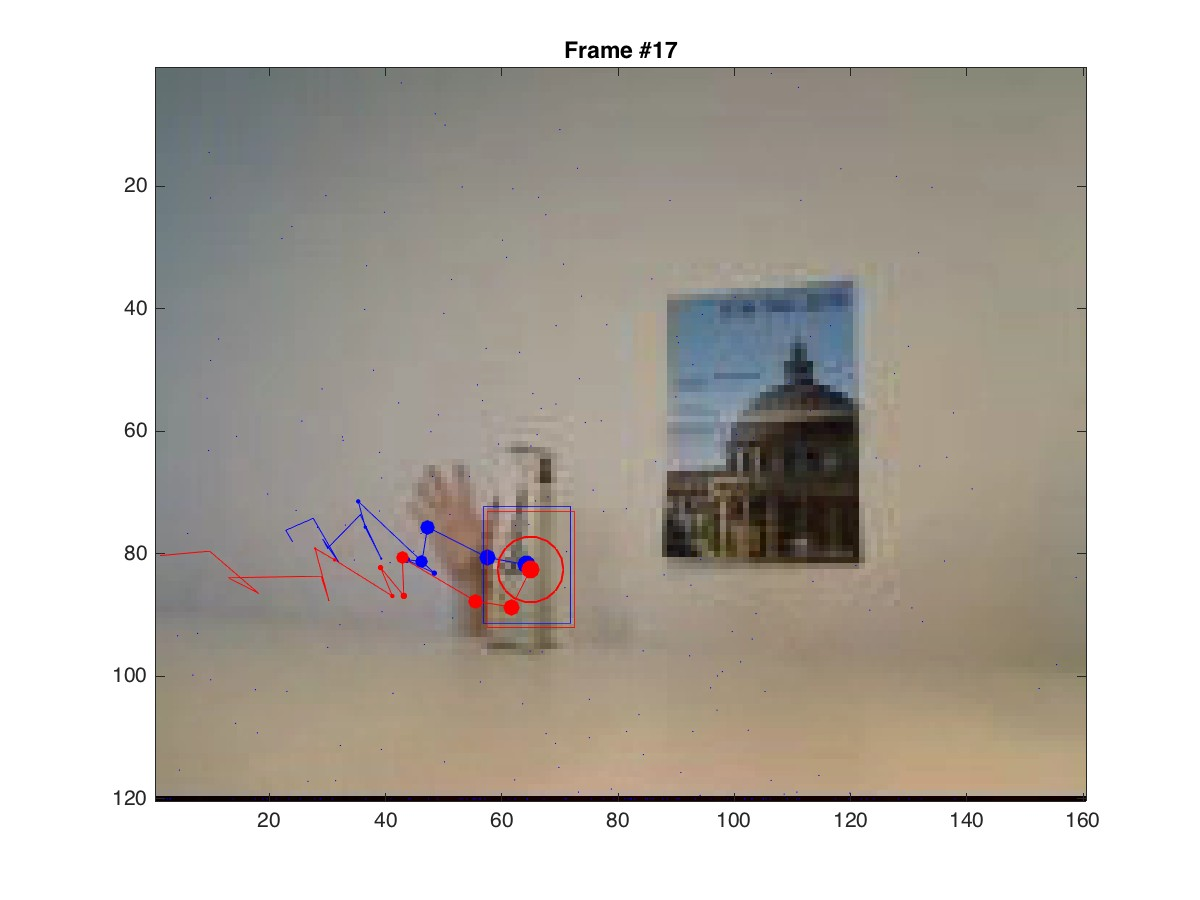
\includegraphics[width=1\linewidth]{images/video2_noise_high_16}
    \end{subfigure}
    \begin{subfigure}[b]{.25\textwidth}
        \centering
        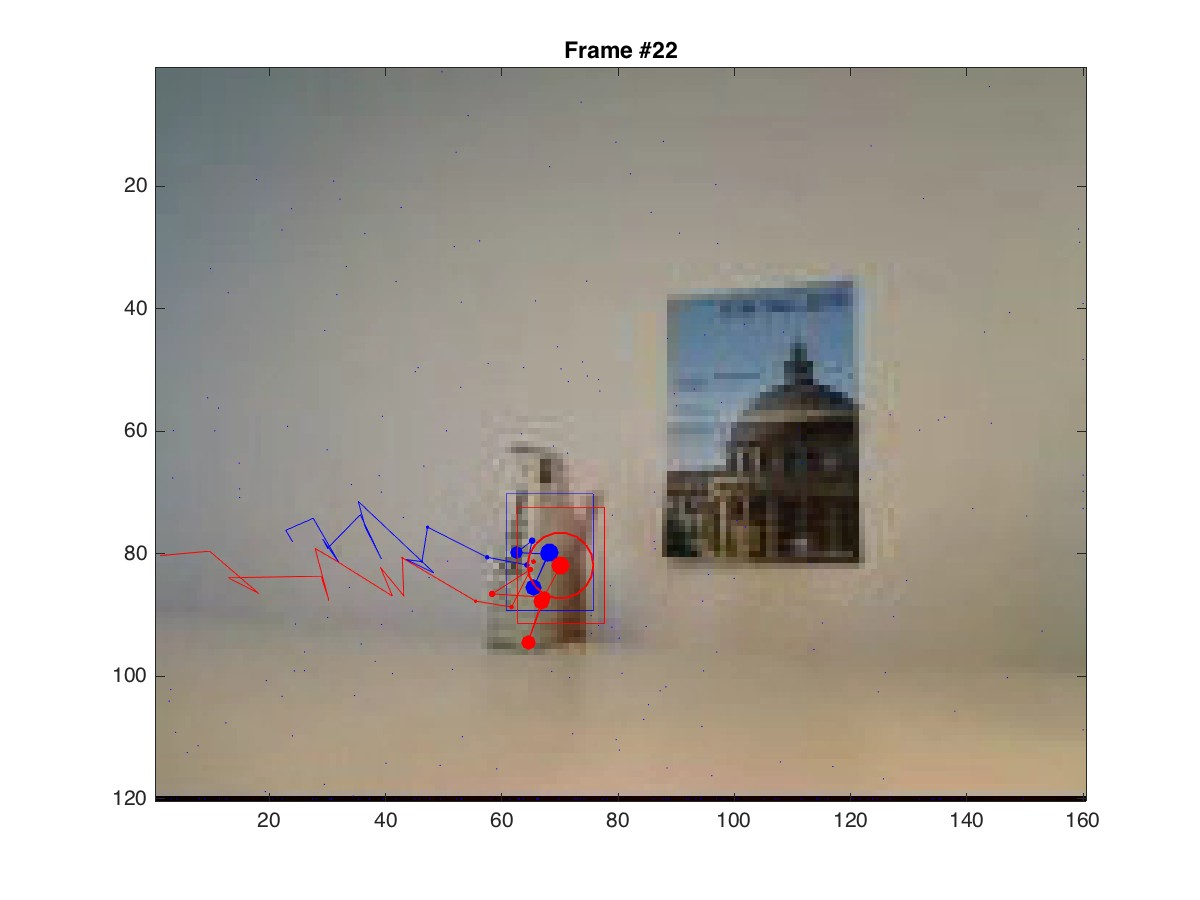
\includegraphics[width=1\linewidth]{images/video2_noise_high_21}
    \end{subfigure}%
    \begin{subfigure}[b]{.25\textwidth}
        \centering
        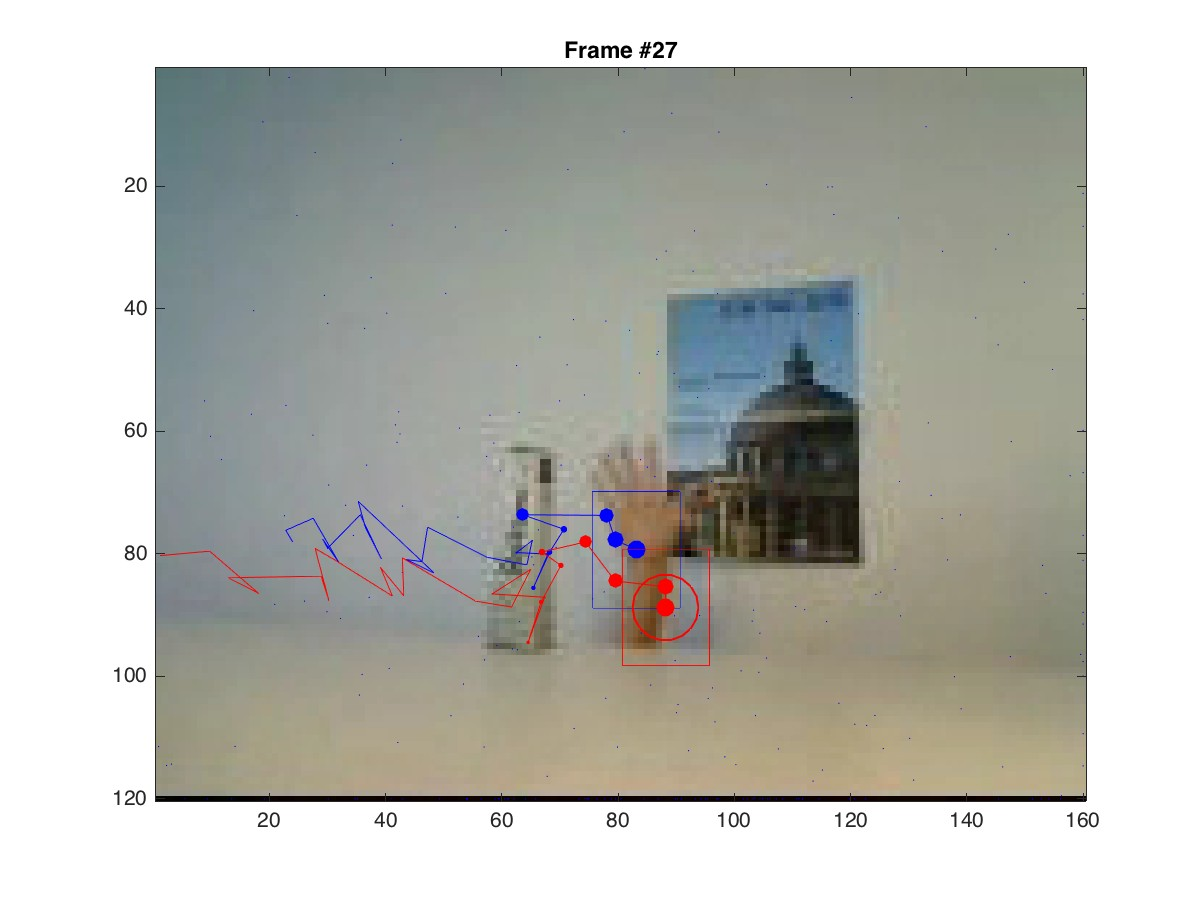
\includegraphics[width=1\linewidth]{images/video2_noise_high_26}
    \end{subfigure}%
    \begin{subfigure}[b]{.25\textwidth}
        \centering
        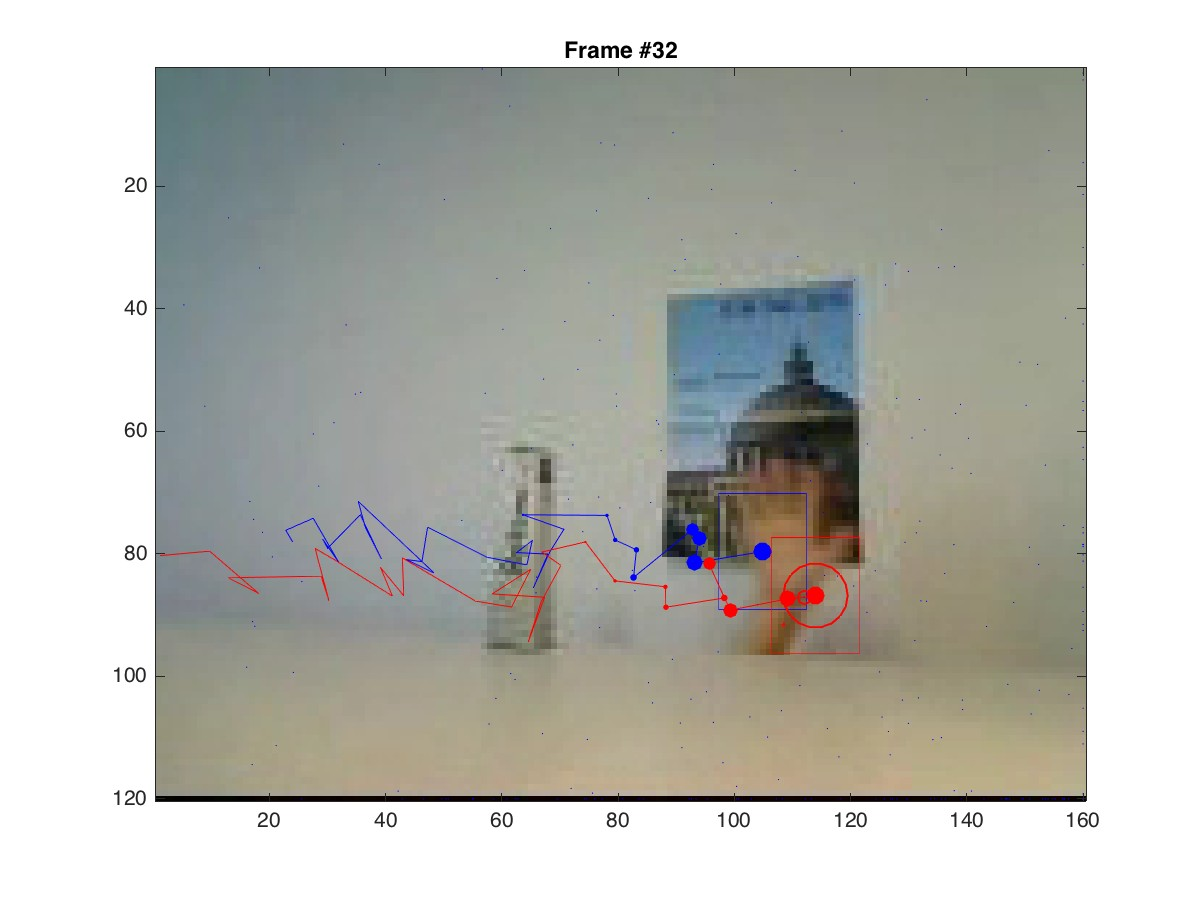
\includegraphics[width=1\linewidth]{images/video2_noise_high_31}
    \end{subfigure}%
    \begin{subfigure}[b]{.25\textwidth}
        \centering
        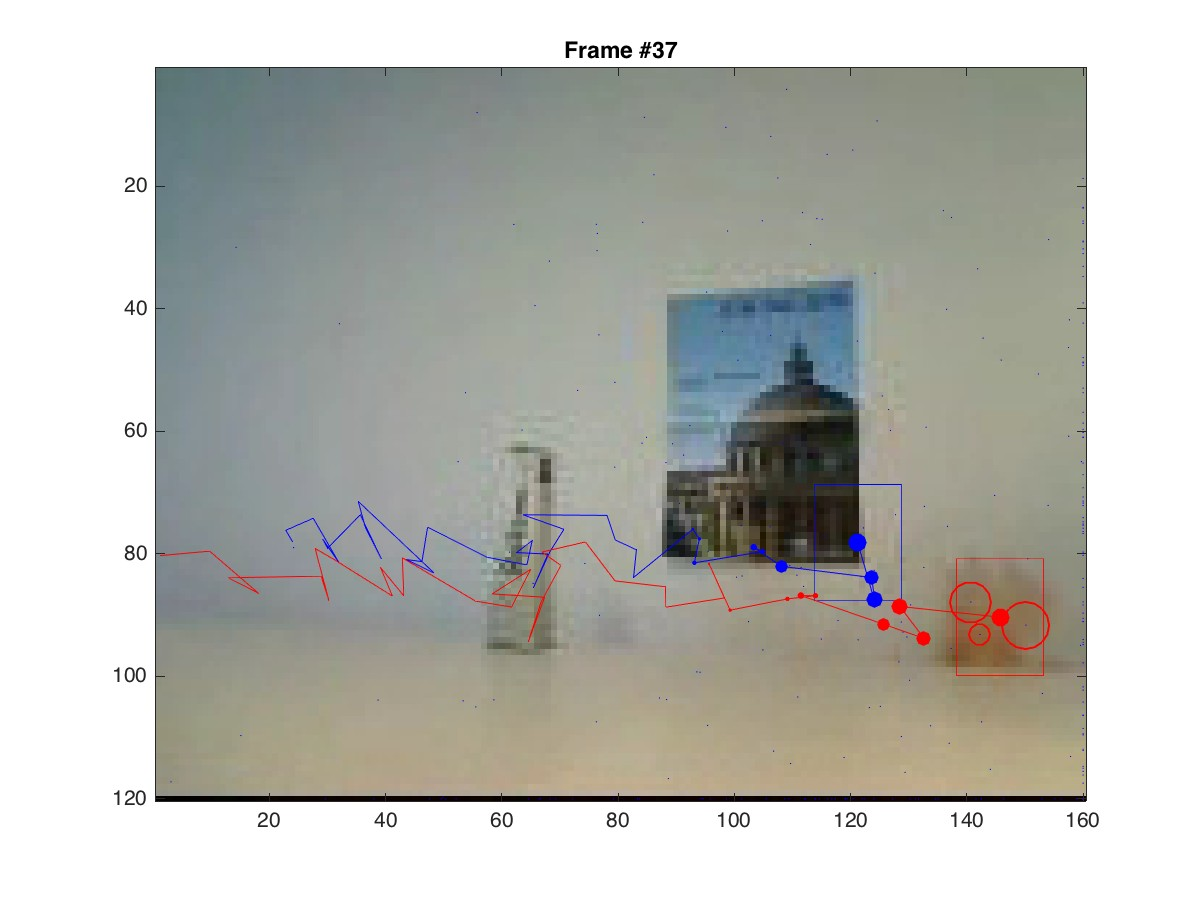
\includegraphics[width=1\linewidth]{images/video2_noise_high_36}
    \end{subfigure}
    \caption{Tracking for \texttt{video2.wmv} with noise $\sigma_{position} = 50$.}
    \label{fig:tracking_video2_noise_high}
\end{figure}

\begin{figure}[h]
    \centering
    \begin{subfigure}[b]{.25\textwidth}
        \centering
        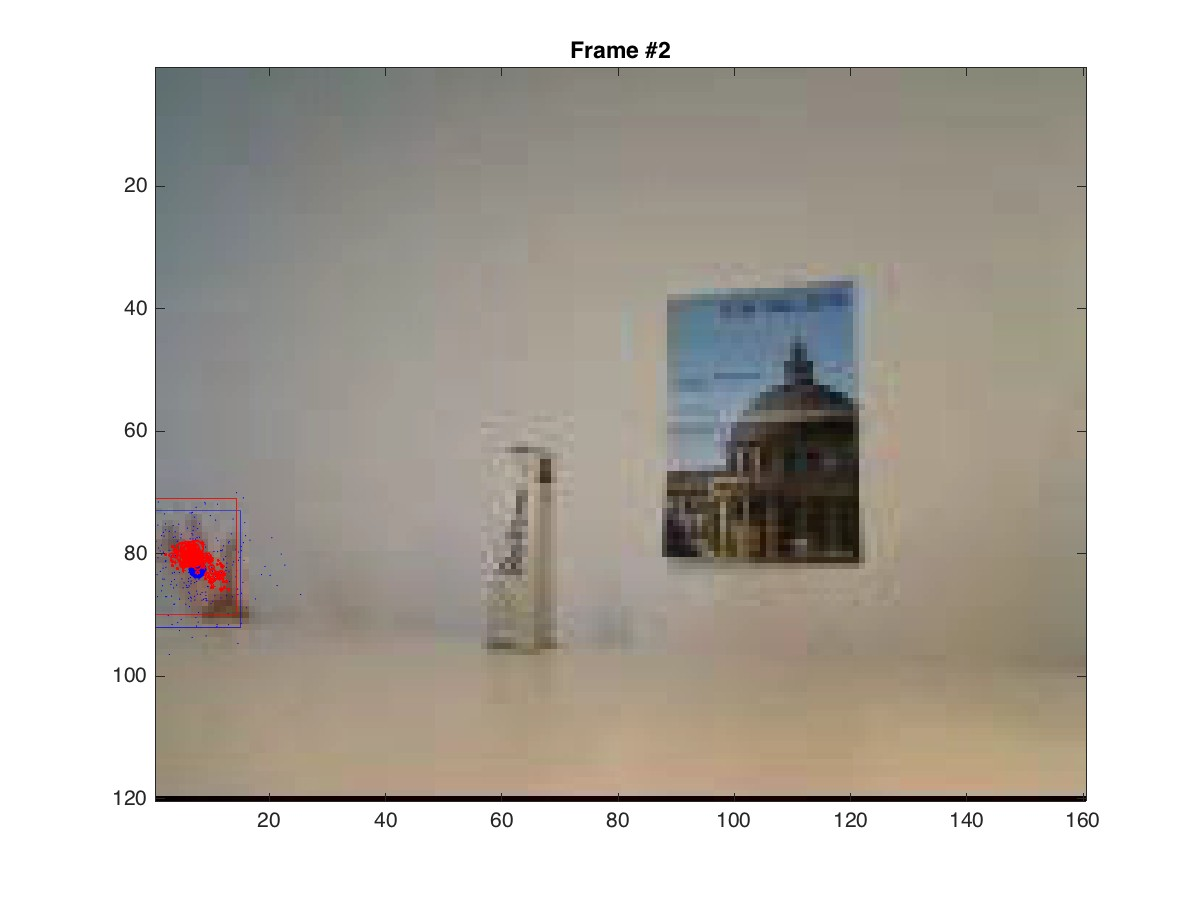
\includegraphics[width=1\linewidth]{images/video2_noise_low_1}
    \end{subfigure}%
    \begin{subfigure}[b]{.25\textwidth}
        \centering
        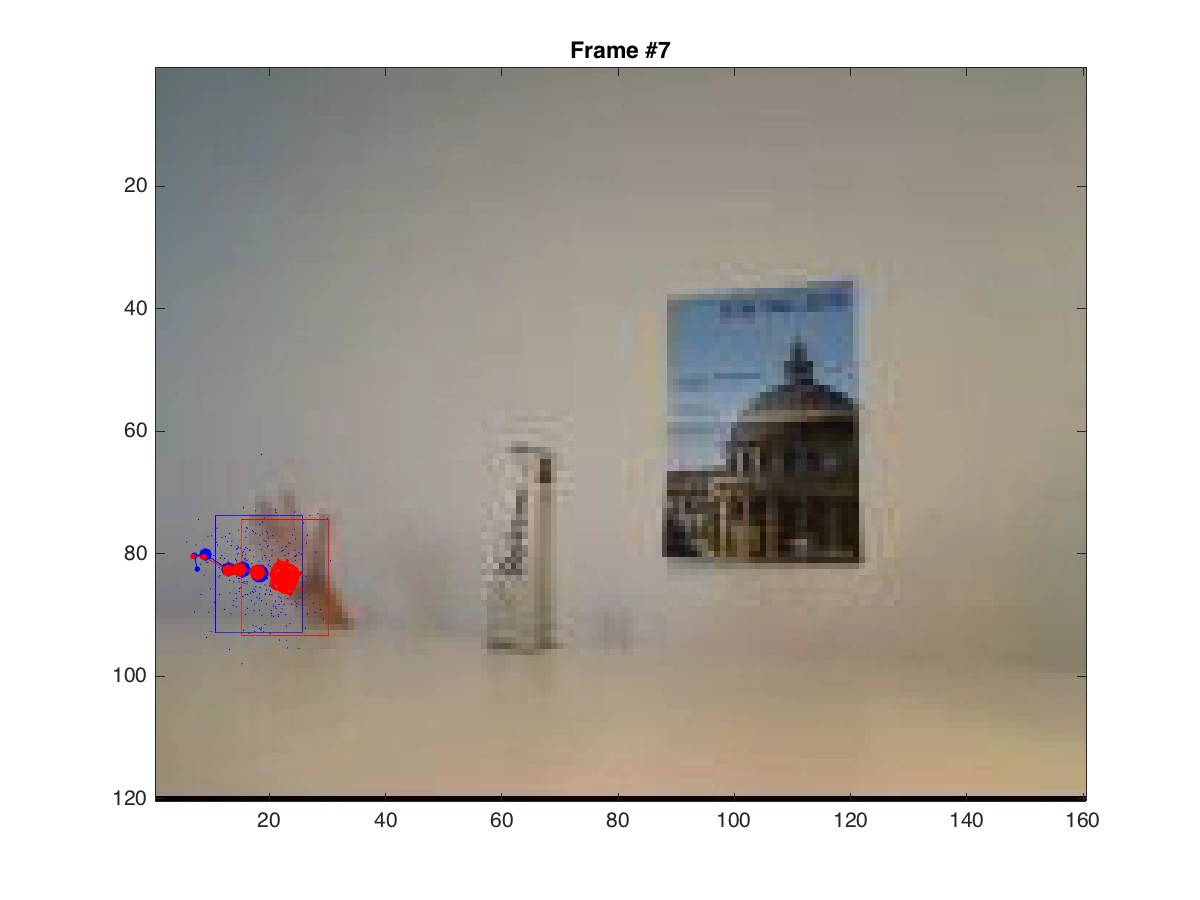
\includegraphics[width=1\linewidth]{images/video2_noise_low_6}
    \end{subfigure}%
    \begin{subfigure}[b]{.25\textwidth}
        \centering
        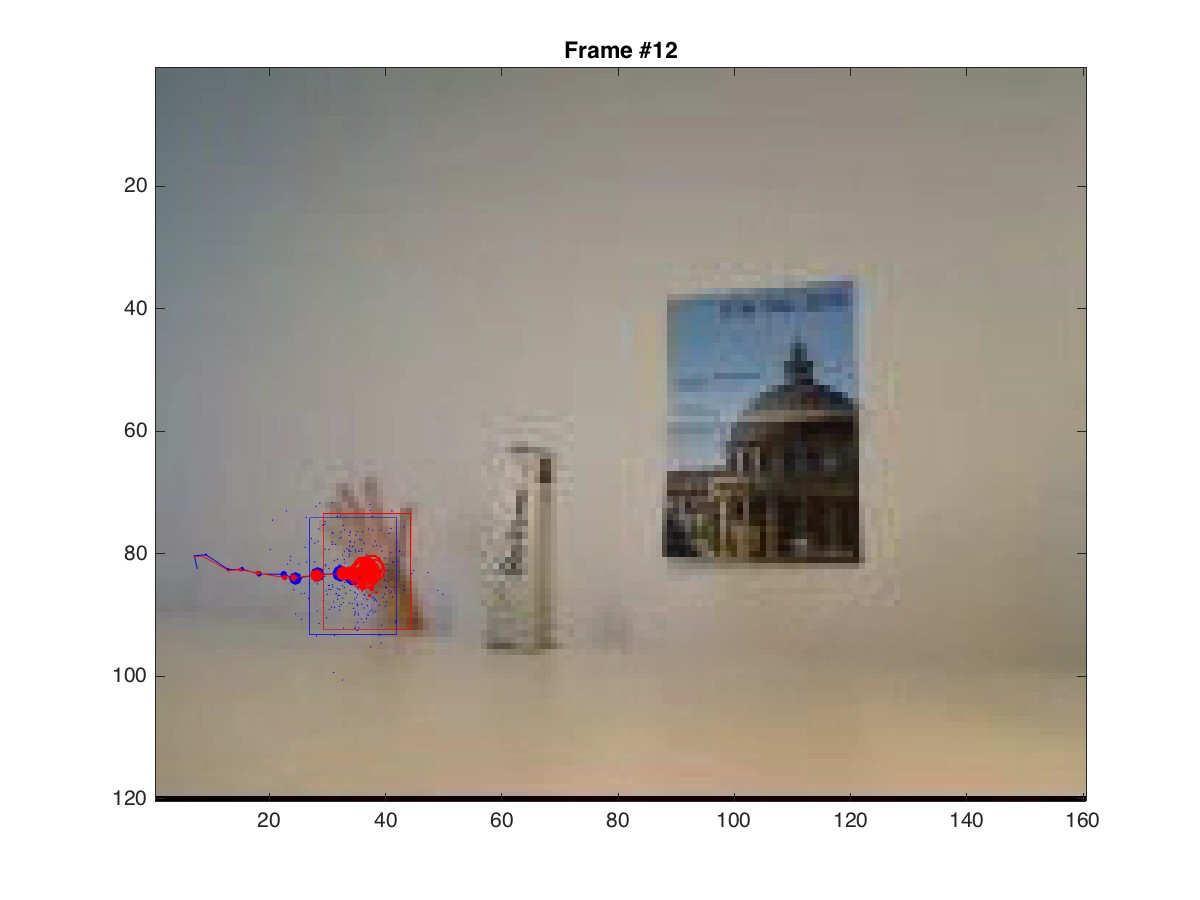
\includegraphics[width=1\linewidth]{images/video2_noise_low_11}
    \end{subfigure}%
    \begin{subfigure}[b]{.25\textwidth}
        \centering
        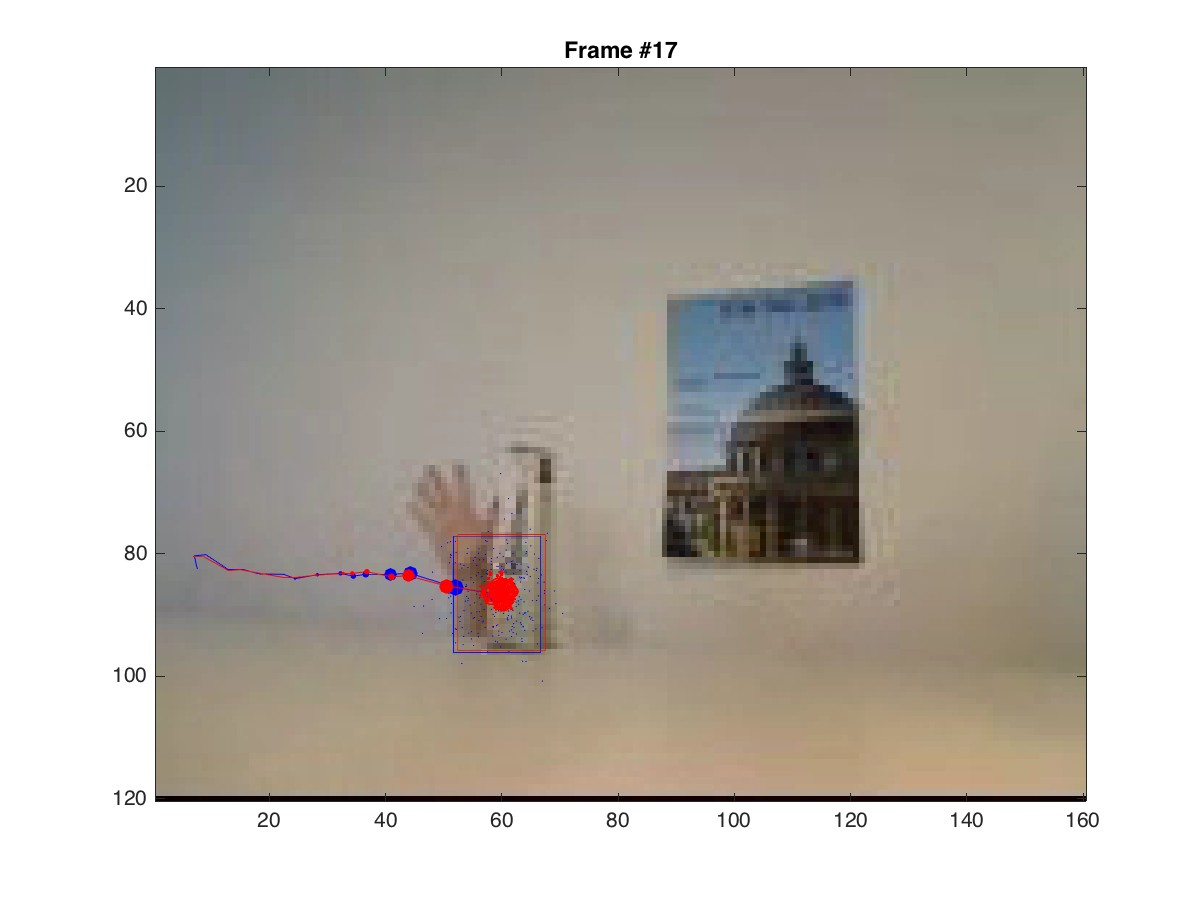
\includegraphics[width=1\linewidth]{images/video2_noise_low_16}
    \end{subfigure}
    \begin{subfigure}[b]{.25\textwidth}
        \centering
        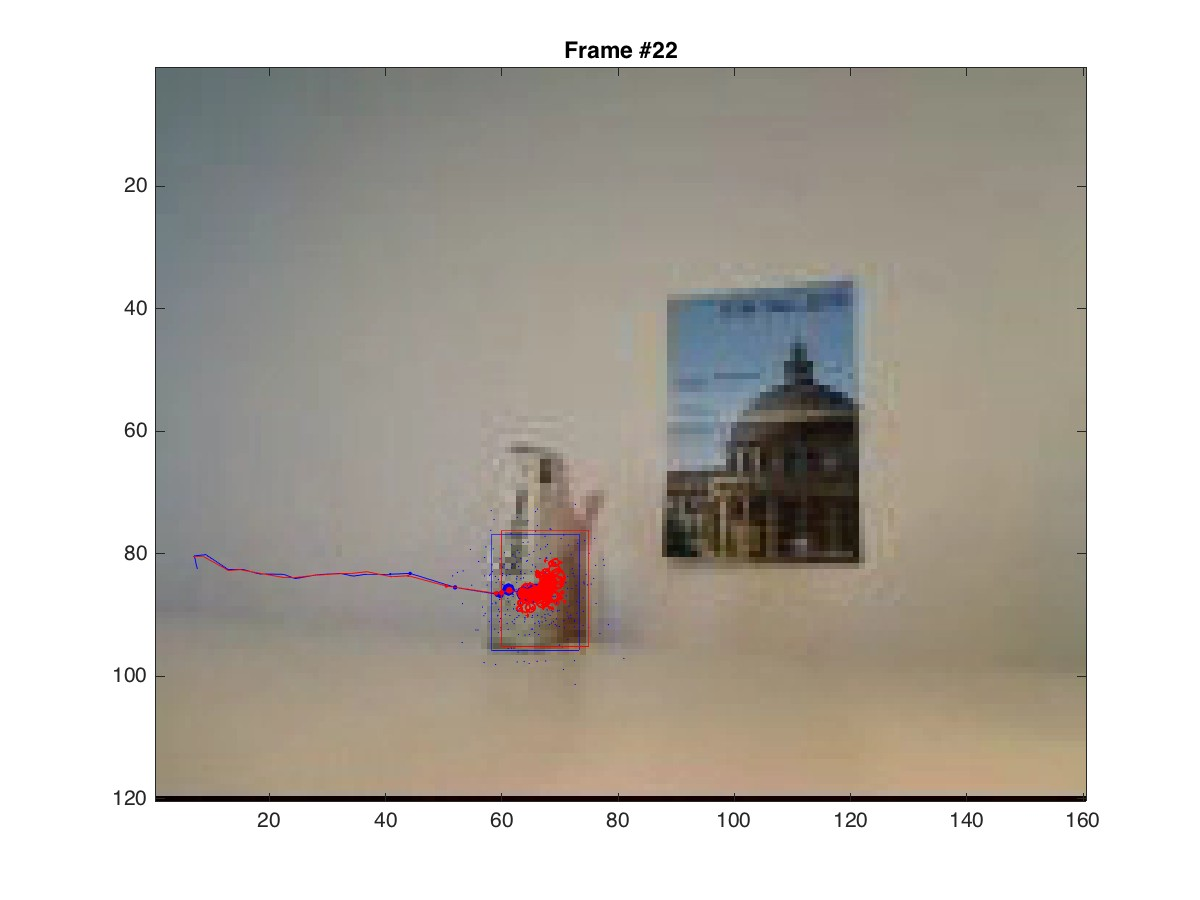
\includegraphics[width=1\linewidth]{images/video2_noise_low_21}
    \end{subfigure}%
    \begin{subfigure}[b]{.25\textwidth}
        \centering
        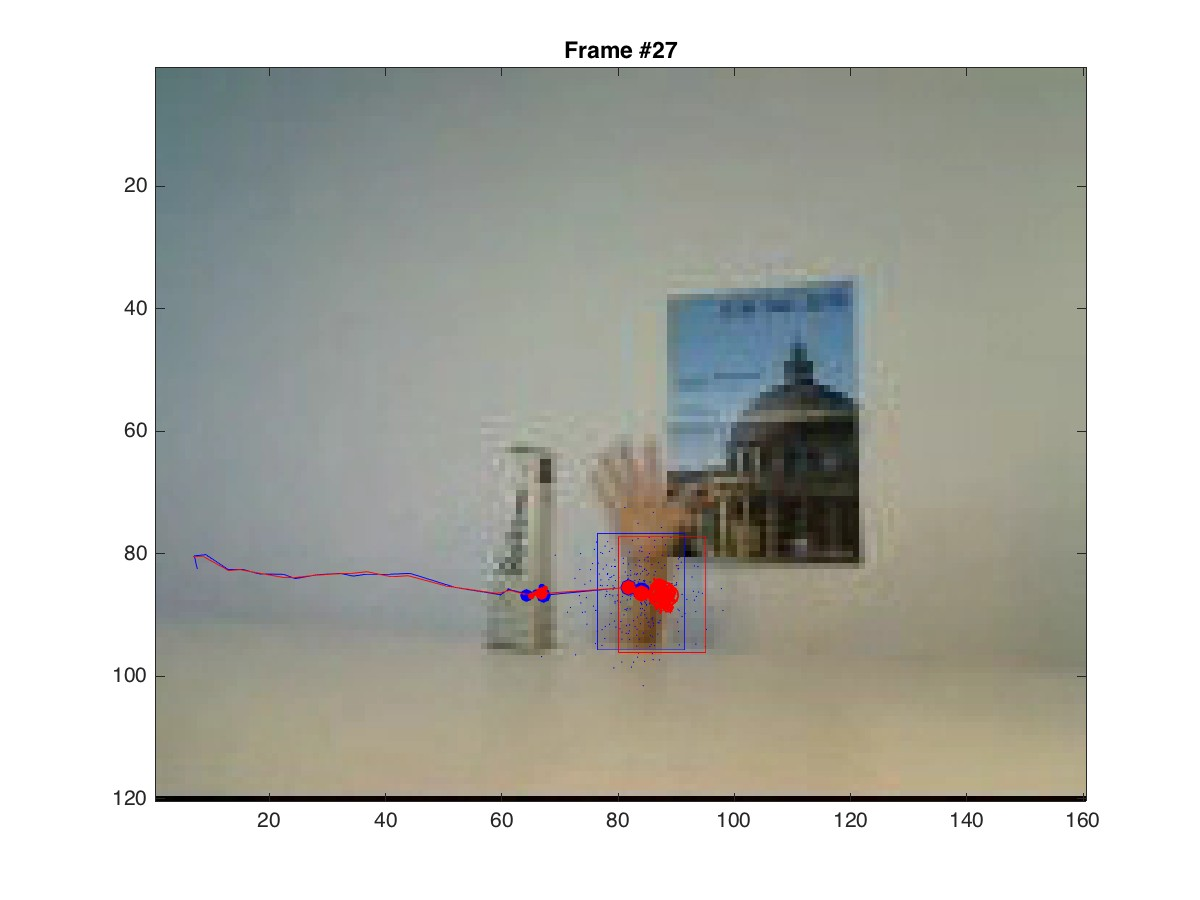
\includegraphics[width=1\linewidth]{images/video2_noise_low_26}
    \end{subfigure}%
    \begin{subfigure}[b]{.25\textwidth}
        \centering
        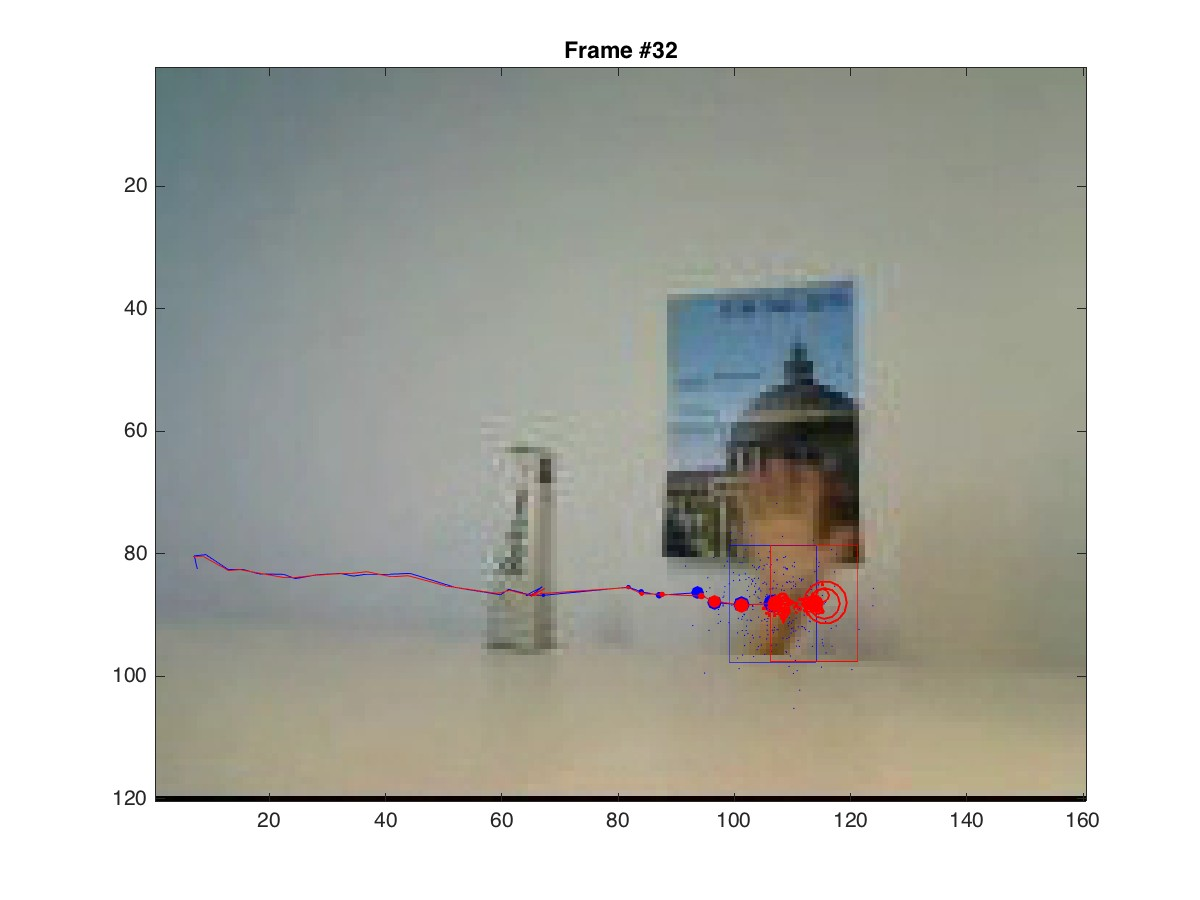
\includegraphics[width=1\linewidth]{images/video2_noise_low_31}
    \end{subfigure}%
    \begin{subfigure}[b]{.25\textwidth}
        \centering
        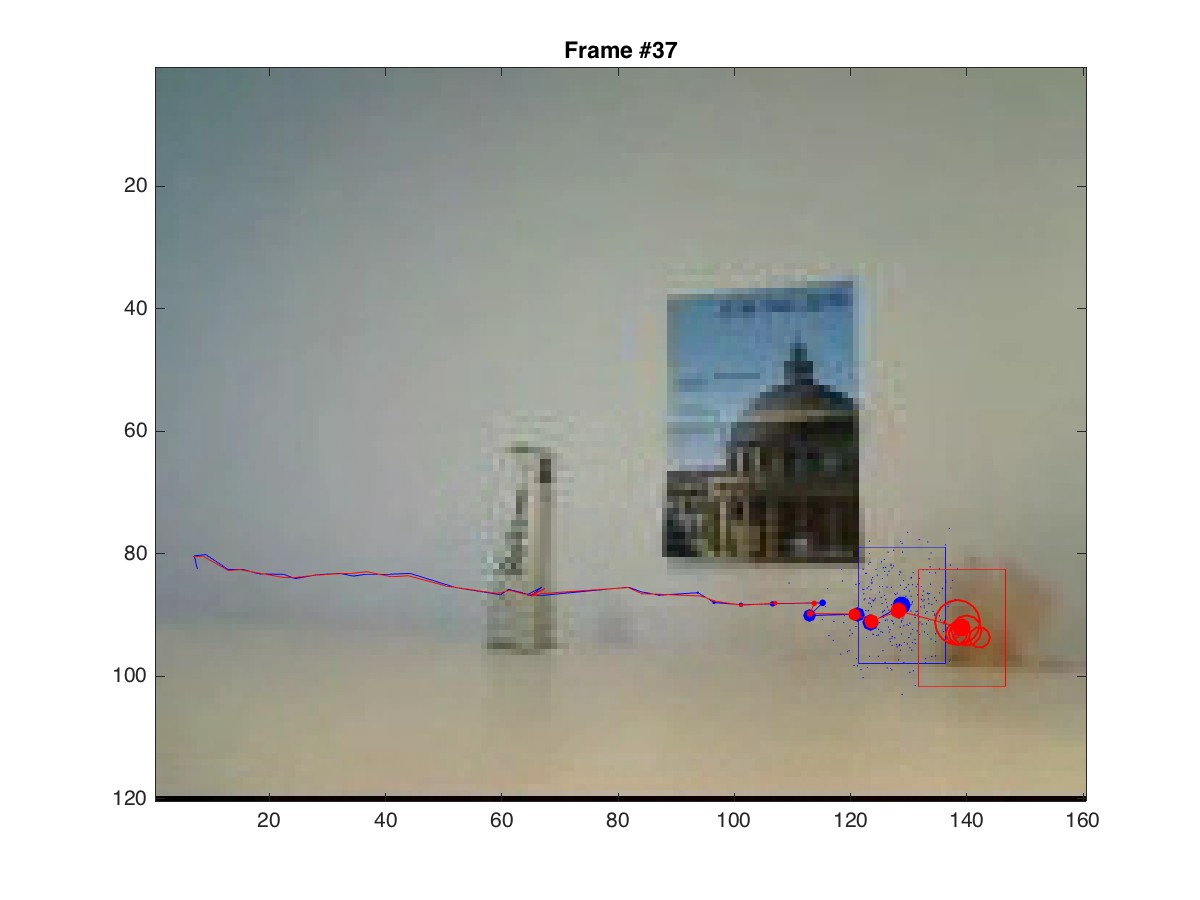
\includegraphics[width=1\linewidth]{images/video2_noise_low_36}
    \end{subfigure}
    \caption{Tracking for \texttt{video2.wmv} with noise $\sigma_{position} = 5$.}
    \label{fig:tracking_video2_noise_low}
\end{figure}

\subsubsection*{Effect of the measurement noise}

Setting back the system noise to the default value ($\sigma_{position} = 15$), it has been tested the effects of the measurement noise into prediction of the Condensation Tracker.
In Figure~\ref{fig:tracking_video2_observe_high} the $\sigma_{observe}$ was set to 1, and it is observe that despite the tracking works well even with the occlusion, the effect is on the values of the particles weights.
As $\sigma_{observe}$ had a high value ($\sigma_{observe} = 1$), the weight for the particles were more spread between them, taking into account more particles than in the default value. On the other hand, setting a small value ($\sigma_{observe} = 0.05$), it can be seen, how only the particle with highest score with its color histogram obtain most of the weight while the rest of the particles do not have any, and so, the posterior prediction of the position goes to this particle.

\begin{figure}[h]
    \centering
    \begin{subfigure}[b]{.25\textwidth}
        \centering
        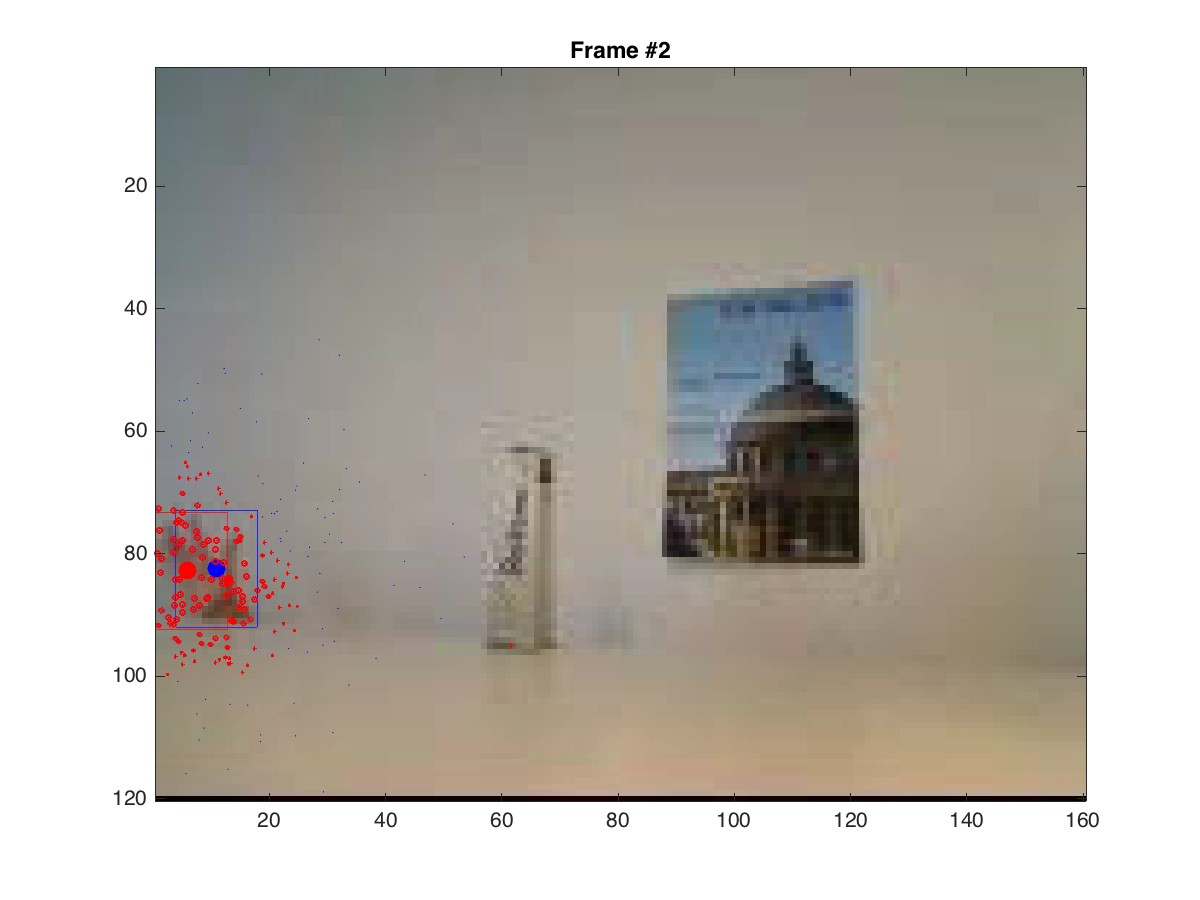
\includegraphics[width=1\linewidth]{images/video2_observe_high_1}
    \end{subfigure}%
    \begin{subfigure}[b]{.25\textwidth}
        \centering
        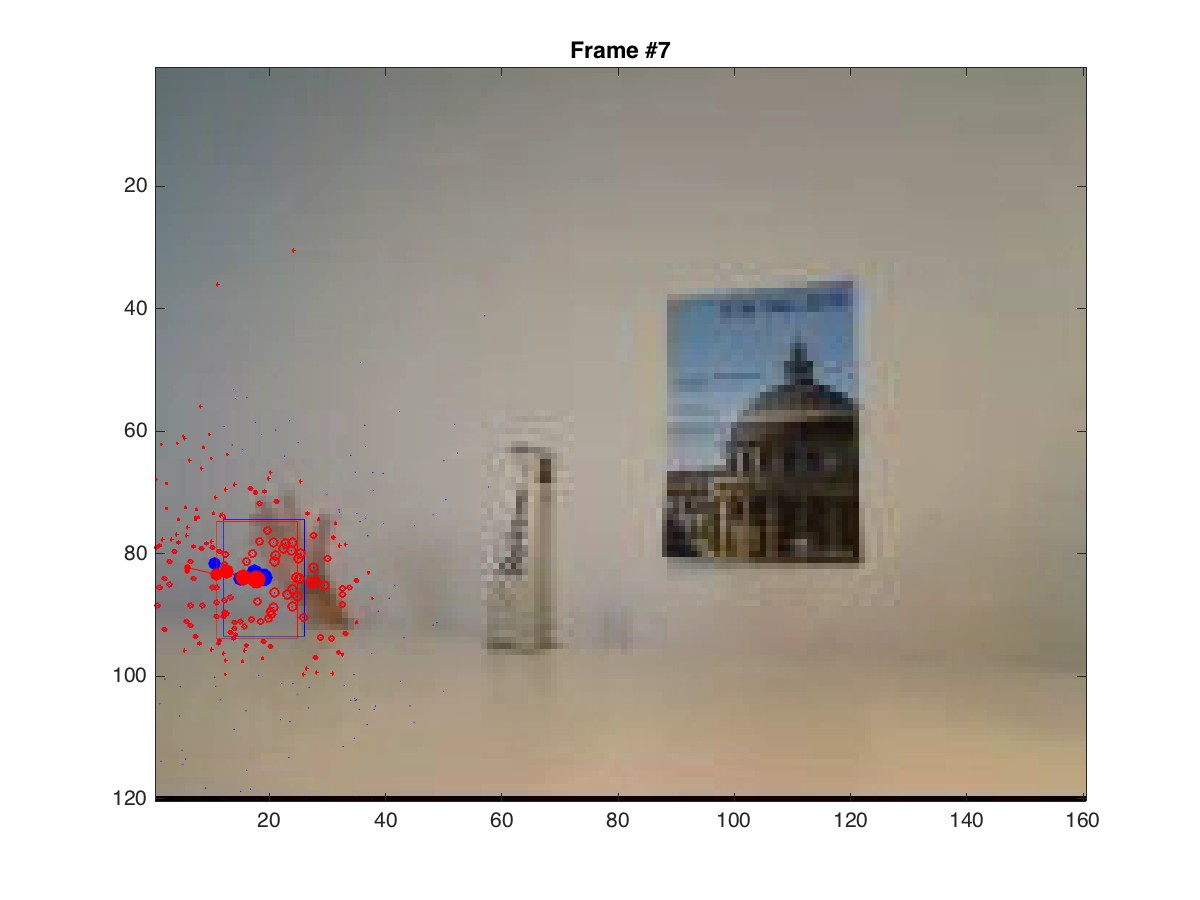
\includegraphics[width=1\linewidth]{images/video2_observe_high_6}
    \end{subfigure}%
    \begin{subfigure}[b]{.25\textwidth}
        \centering
        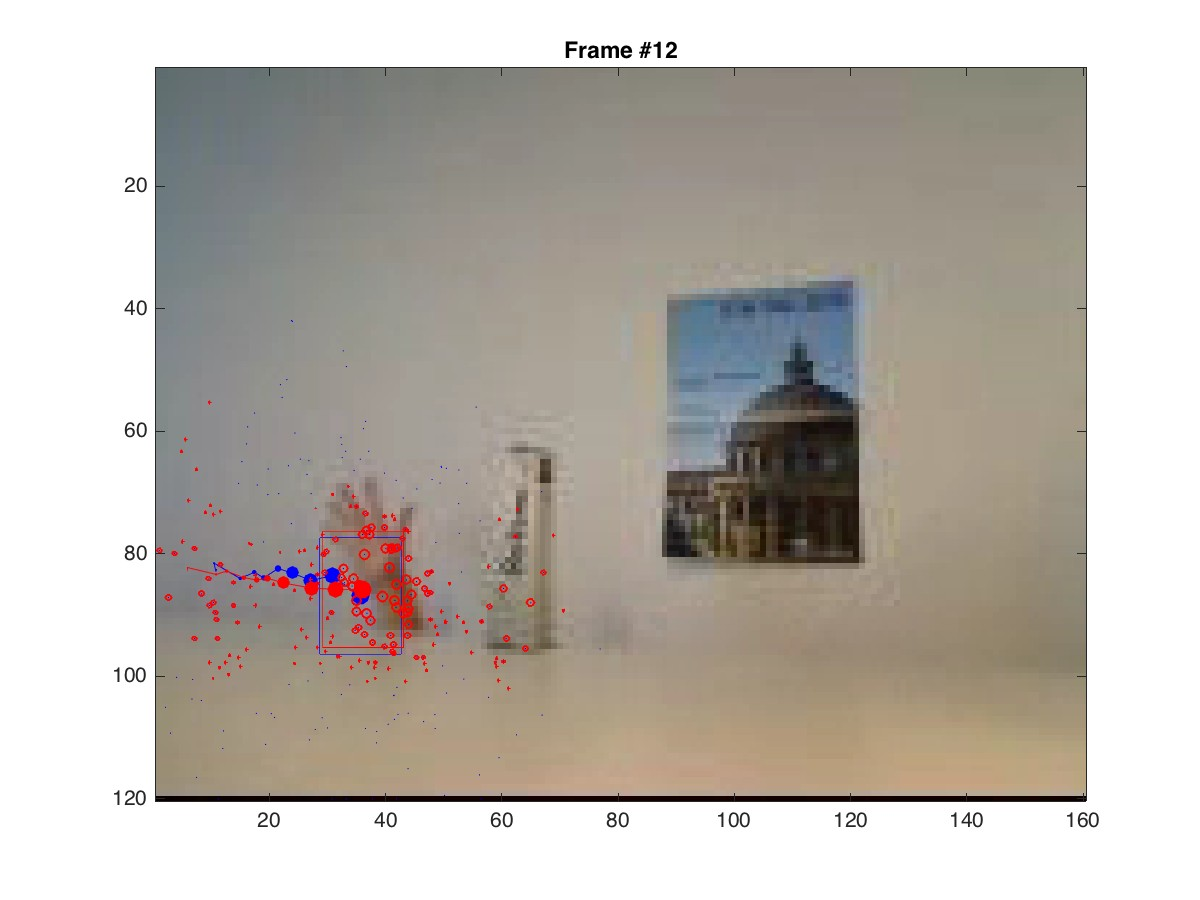
\includegraphics[width=1\linewidth]{images/video2_observe_high_11}
    \end{subfigure}%
    \begin{subfigure}[b]{.25\textwidth}
        \centering
        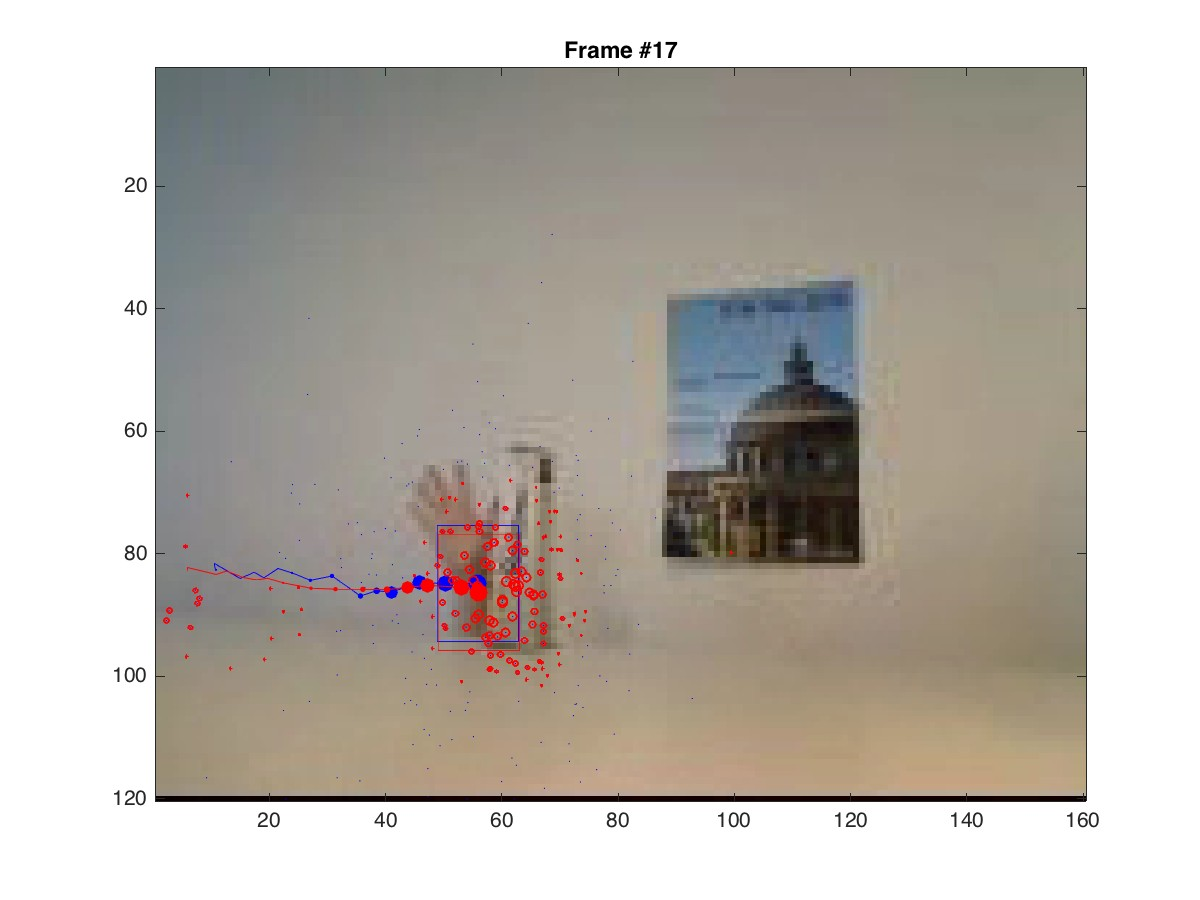
\includegraphics[width=1\linewidth]{images/video2_observe_high_16}
    \end{subfigure}
    \begin{subfigure}[b]{.25\textwidth}
        \centering
        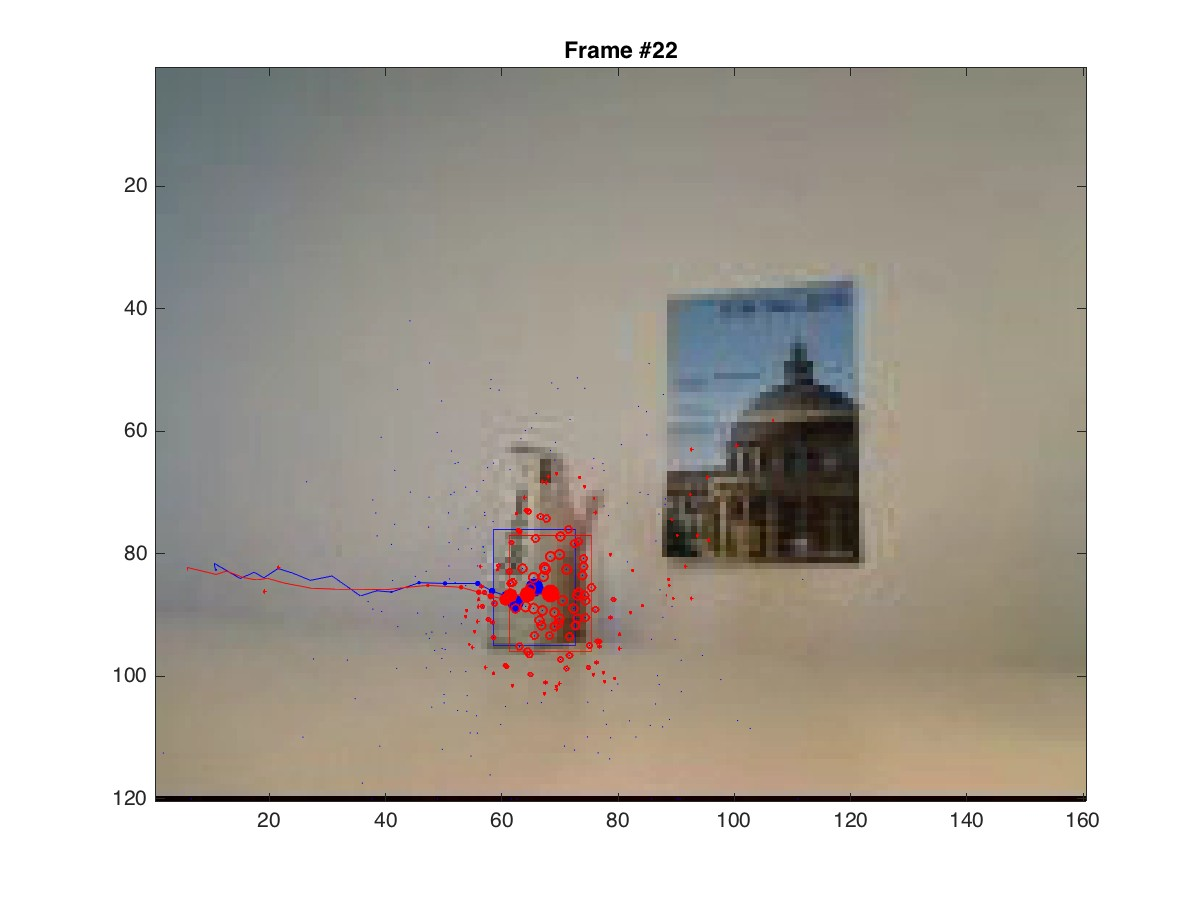
\includegraphics[width=1\linewidth]{images/video2_observe_high_21}
    \end{subfigure}%
    \begin{subfigure}[b]{.25\textwidth}
        \centering
        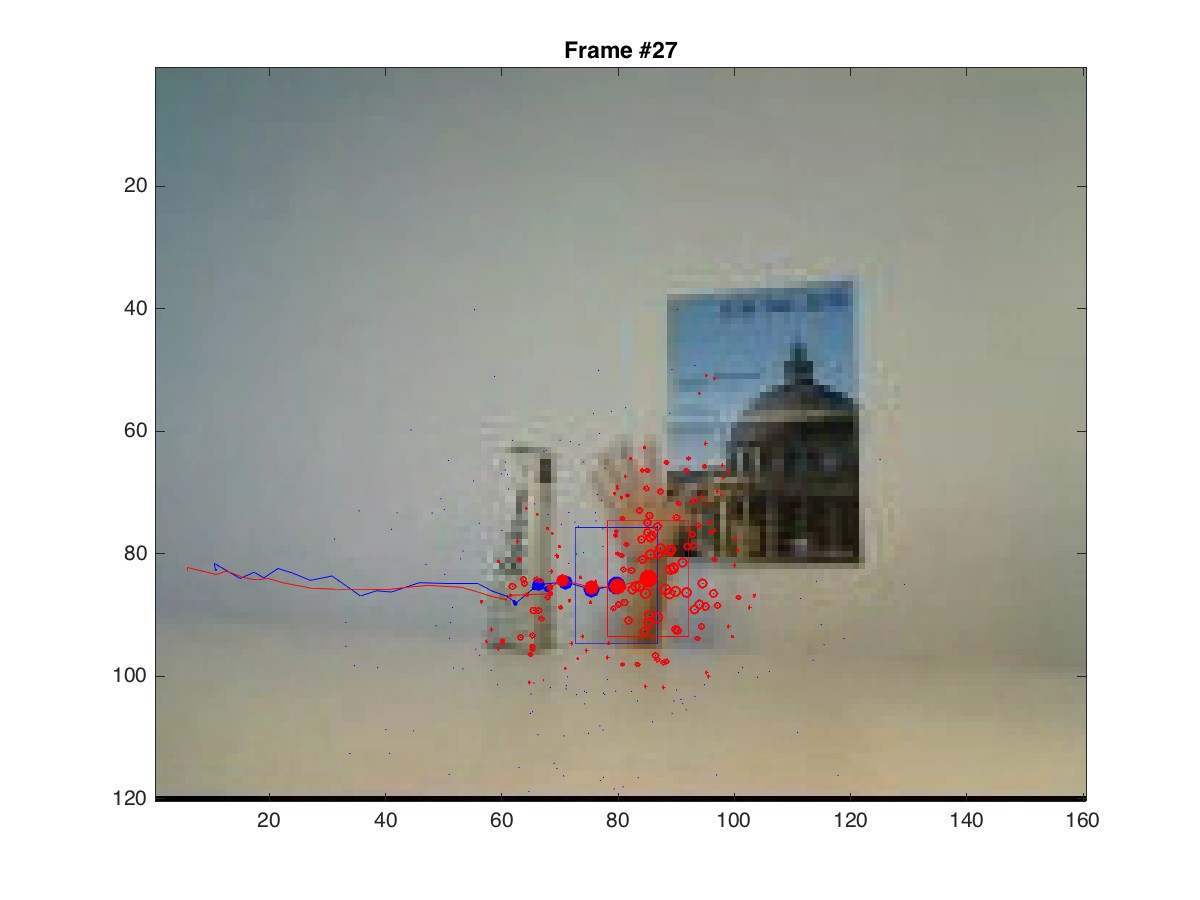
\includegraphics[width=1\linewidth]{images/video2_observe_high_26}
    \end{subfigure}%
    \begin{subfigure}[b]{.25\textwidth}
        \centering
        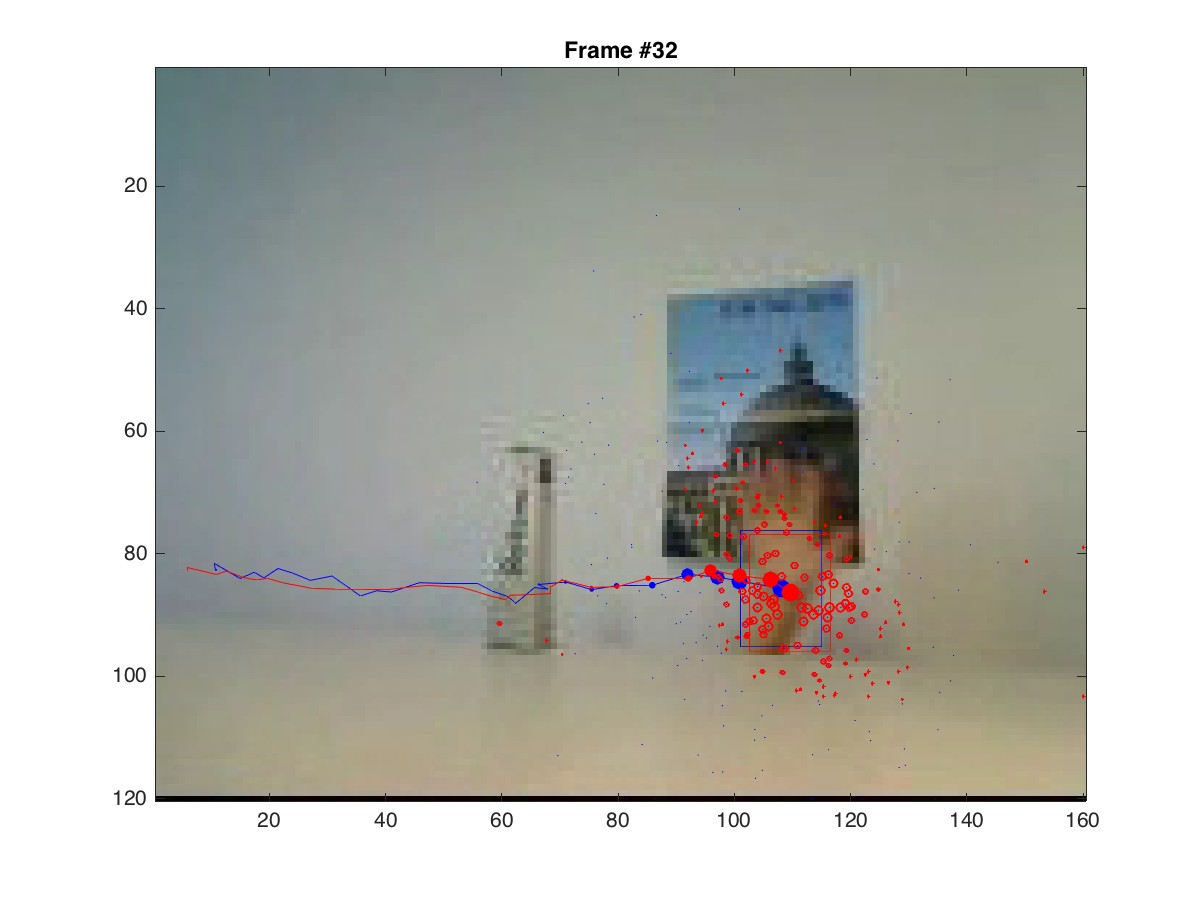
\includegraphics[width=1\linewidth]{images/video2_observe_high_31}
    \end{subfigure}%
    \begin{subfigure}[b]{.25\textwidth}
        \centering
        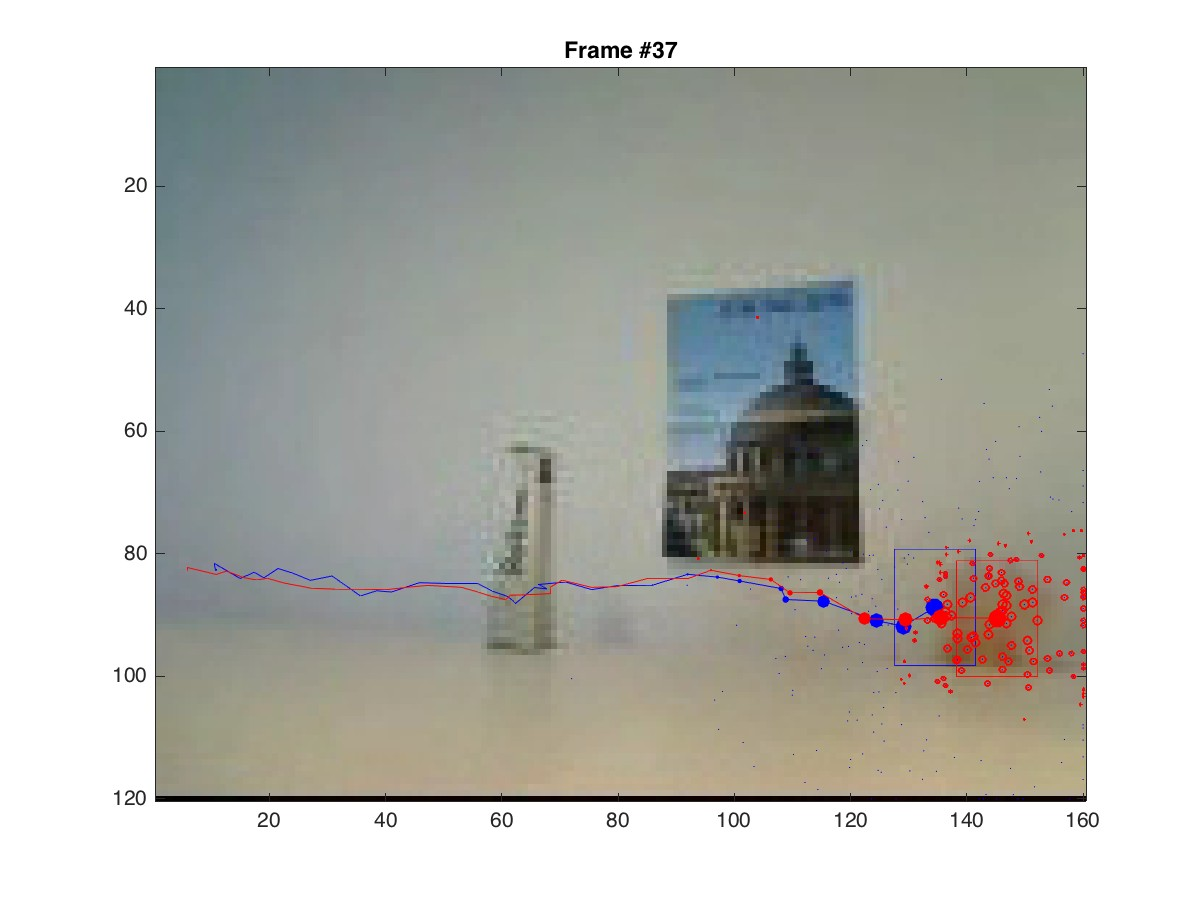
\includegraphics[width=1\linewidth]{images/video2_observe_high_36}
    \end{subfigure}
    \caption{Tracking for \texttt{video2.wmv} with noise $\sigma_{observe} = 1$.}
    \label{fig:tracking_video2_observe_high}
\end{figure}

\begin{figure}[h]
    \centering
    \begin{subfigure}[b]{.25\textwidth}
        \centering
        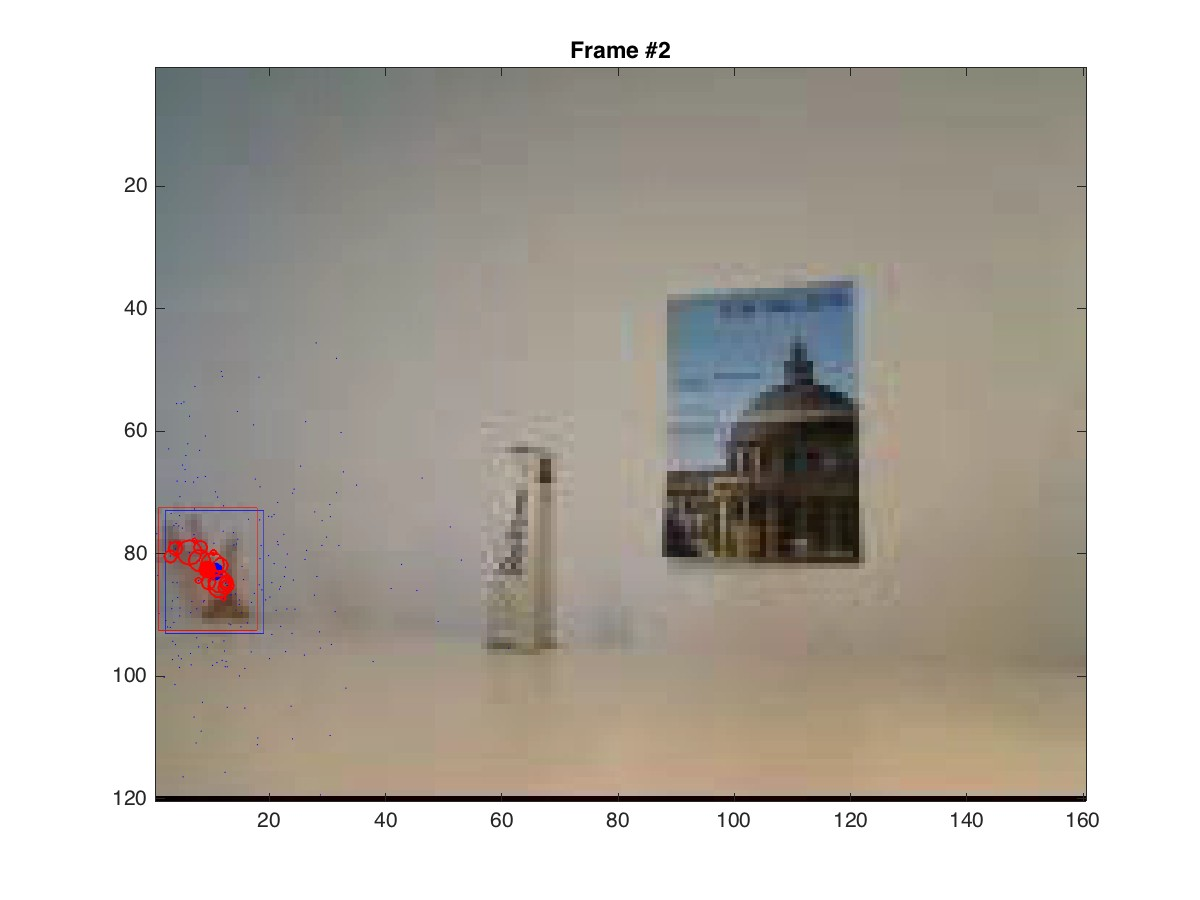
\includegraphics[width=1\linewidth]{images/video2_observe_low_1}
    \end{subfigure}%
    \begin{subfigure}[b]{.25\textwidth}
        \centering
        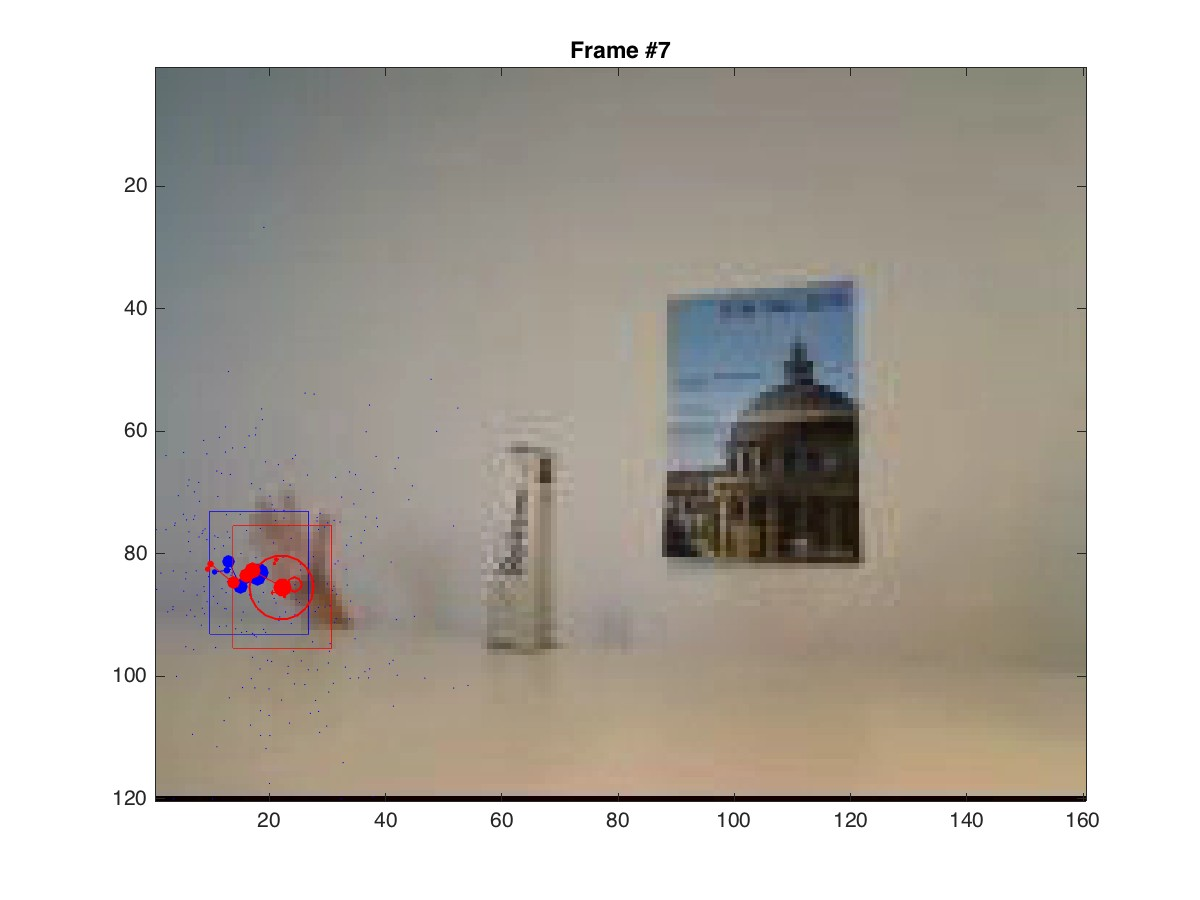
\includegraphics[width=1\linewidth]{images/video2_observe_low_6}
    \end{subfigure}%
    \begin{subfigure}[b]{.25\textwidth}
        \centering
        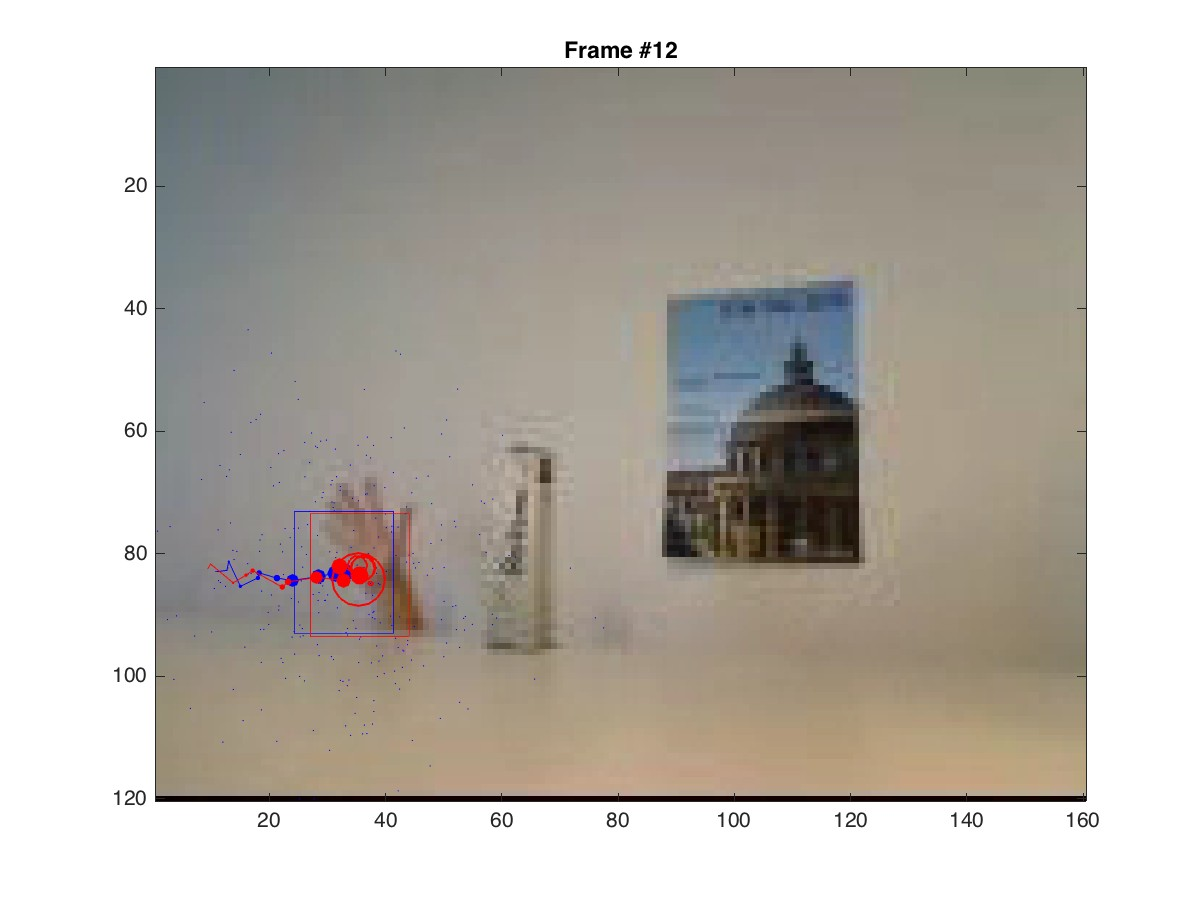
\includegraphics[width=1\linewidth]{images/video2_observe_low_11}
    \end{subfigure}%
    \begin{subfigure}[b]{.25\textwidth}
        \centering
        \includegraphics[width=1\linewidth]{images/video2_observe_low_16}
    \end{subfigure}
    \begin{subfigure}[b]{.25\textwidth}
        \centering
        \includegraphics[width=1\linewidth]{images/video2_observe_low_21}
    \end{subfigure}%
    \begin{subfigure}[b]{.25\textwidth}
        \centering
        \includegraphics[width=1\linewidth]{images/video2_observe_low_26}
    \end{subfigure}%
    \begin{subfigure}[b]{.25\textwidth}
        \centering
        \includegraphics[width=1\linewidth]{images/video2_observe_low_31}
    \end{subfigure}%
    \begin{subfigure}[b]{.25\textwidth}
        \centering
        \includegraphics[width=1\linewidth]{images/video2_observe_low_36}
    \end{subfigure}
    \caption{Tracking for \texttt{video2.wmv} with observe $\sigma_{observe} = 0.05$.}
    \label{fig:tracking_video2_observe_low}
\end{figure}

\subsection*{\texttt{video3.wmv}}

For the third video, the same parameters are going to be used as in \texttt{video2.wmv} and only the remarkable facts are going to be commented.

\begin{figure}[h]
    \centering
    \begin{subfigure}[b]{.25\textwidth}
        \centering
        \includegraphics[width=1\linewidth]{images/video3__1}
    \end{subfigure}%
    \begin{subfigure}[b]{.25\textwidth}
        \centering
        \includegraphics[width=1\linewidth]{images/video3__6}
    \end{subfigure}%
    \begin{subfigure}[b]{.25\textwidth}
        \centering
        \includegraphics[width=1\linewidth]{images/video3__11}
    \end{subfigure}%
    \begin{subfigure}[b]{.25\textwidth}
        \centering
        \includegraphics[width=1\linewidth]{images/video3__16}
    \end{subfigure}
    \begin{subfigure}[b]{.25\textwidth}
        \centering
        \includegraphics[width=1\linewidth]{images/video3__21}
    \end{subfigure}%
    \begin{subfigure}[b]{.25\textwidth}
        \centering
        \includegraphics[width=1\linewidth]{images/video3__26}
    \end{subfigure}%
    \begin{subfigure}[b]{.25\textwidth}
        \centering
        \includegraphics[width=1\linewidth]{images/video3__31}
    \end{subfigure}%
    \begin{subfigure}[b]{.25\textwidth}
        \centering
        \includegraphics[width=1\linewidth]{images/video3__36}
    \end{subfigure}
    \begin{subfigure}[b]{.25\textwidth}
        \centering
        \includegraphics[width=1\linewidth]{images/video3__41}
    \end{subfigure}%
    \begin{subfigure}[b]{.25\textwidth}
        \centering
        \includegraphics[width=1\linewidth]{images/video3__46}
    \end{subfigure}%
    \begin{subfigure}[b]{.25\textwidth}
        \centering
        \includegraphics[width=1\linewidth]{images/video3__51}
    \end{subfigure}%
    \begin{subfigure}[b]{.25\textwidth}
        \centering
        \includegraphics[width=1\linewidth]{images/video3__56}
    \end{subfigure}
    \caption{Tracking of the ball at \texttt{video3.wmv} using the implemented Condensation Tracker with default values}
    \label{fig:tracking_video3}
\end{figure}

\subsubsection*{Effect of the model}

In Figure~\ref{fig:tracking_video3_model} can be seen how setting a constant velocity model, with $v_0 = [10,1]^T$, the tracking works well but there is sometimes a lot of difference between the prior prediction of the position and the posterior. As it is assuming a constant velocity to the right, when the ball come to the left after touching the wall, the prior prediction starts to look far from the true position, so in this case, with an object moving in two different direction along the video, its not recommendable to use a model that assumes constant velocity for the object to track.

\begin{figure}[h]
    \centering
    \begin{subfigure}[b]{.25\textwidth}
        \centering
        \includegraphics[width=1\linewidth]{images/video3_model_1}
    \end{subfigure}%
    \begin{subfigure}[b]{.25\textwidth}
        \centering
        \includegraphics[width=1\linewidth]{images/video3_model_6}
    \end{subfigure}%
    \begin{subfigure}[b]{.25\textwidth}
        \centering
        \includegraphics[width=1\linewidth]{images/video3_model_11}
    \end{subfigure}%
    \begin{subfigure}[b]{.25\textwidth}
        \centering
        \includegraphics[width=1\linewidth]{images/video3_model_16}
    \end{subfigure}
    \begin{subfigure}[b]{.25\textwidth}
        \centering
        \includegraphics[width=1\linewidth]{images/video3_model_21}
    \end{subfigure}%
    \begin{subfigure}[b]{.25\textwidth}
        \centering
        \includegraphics[width=1\linewidth]{images/video3_model_26}
    \end{subfigure}%
    \begin{subfigure}[b]{.25\textwidth}
        \centering
        \includegraphics[width=1\linewidth]{images/video3_model_31}
    \end{subfigure}%
    \begin{subfigure}[b]{.25\textwidth}
        \centering
        \includegraphics[width=1\linewidth]{images/video3_model_36}
    \end{subfigure}
    \begin{subfigure}[b]{.25\textwidth}
        \centering
        \includegraphics[width=1\linewidth]{images/video3_model_41}
    \end{subfigure}%
    \begin{subfigure}[b]{.25\textwidth}
        \centering
        \includegraphics[width=1\linewidth]{images/video3_model_46}
    \end{subfigure}%
    \begin{subfigure}[b]{.25\textwidth}
        \centering
        \includegraphics[width=1\linewidth]{images/video3_model_51}
    \end{subfigure}%
    \begin{subfigure}[b]{.25\textwidth}
        \centering
        \includegraphics[width=1\linewidth]{images/video3_model_56}
    \end{subfigure}
    \caption{Tracking for \texttt{video3.wmv} with the constant velocity model.}
    \label{fig:tracking_video3_model}
\end{figure}

\subsubsection*{Effect of the system noise}

Changing the system noise, it can be seen that setting a $\sigma_{position}$ a little bit higher than the default, happens that in a certain point of the video, some particle lay over the bottom right zone of the frame where the histogram obtain more match and the tracker loose the track of the ball (Figure~\ref{fig:tracking_video3_noise_high}). On the other hand, setting a smaller $\sigma_{position}$, the particles keep closer to the object to track (as it doesn't move so fast) and predict a smoother tracking of the ball (Figure~\ref{fig:tracking_video3_noise_low}).

\begin{figure}[h]
    \centering
    \begin{subfigure}[b]{.25\textwidth}
        \centering
        \includegraphics[width=1\linewidth]{images/video3_noise_high_1}
    \end{subfigure}%
    \begin{subfigure}[b]{.25\textwidth}
        \centering
        \includegraphics[width=1\linewidth]{images/video3_noise_high_6}
    \end{subfigure}%
    \begin{subfigure}[b]{.25\textwidth}
        \centering
        \includegraphics[width=1\linewidth]{images/video3_noise_high_11}
    \end{subfigure}%
    \begin{subfigure}[b]{.25\textwidth}
        \centering
        \includegraphics[width=1\linewidth]{images/video3_noise_high_16}
    \end{subfigure}
    \begin{subfigure}[b]{.25\textwidth}
        \centering
        \includegraphics[width=1\linewidth]{images/video3_noise_high_21}
    \end{subfigure}%
    \begin{subfigure}[b]{.25\textwidth}
        \centering
        \includegraphics[width=1\linewidth]{images/video3_noise_high_26}
    \end{subfigure}%
    \begin{subfigure}[b]{.25\textwidth}
        \centering
        \includegraphics[width=1\linewidth]{images/video3_noise_high_31}
    \end{subfigure}%
    \begin{subfigure}[b]{.25\textwidth}
        \centering
        \includegraphics[width=1\linewidth]{images/video3_noise_high_36}
    \end{subfigure}
    \begin{subfigure}[b]{.25\textwidth}
        \centering
        \includegraphics[width=1\linewidth]{images/video3_noise_high_41}
    \end{subfigure}%
    \begin{subfigure}[b]{.25\textwidth}
        \centering
        \includegraphics[width=1\linewidth]{images/video3_noise_high_46}
    \end{subfigure}%
    \begin{subfigure}[b]{.25\textwidth}
        \centering
        \includegraphics[width=1\linewidth]{images/video3_noise_high_51}
    \end{subfigure}%
    \begin{subfigure}[b]{.25\textwidth}
        \centering
        \includegraphics[width=1\linewidth]{images/video3_noise_high_56}
    \end{subfigure}
    \caption{Tracking for \texttt{video3.wmv} with the $\sigma_{position} = 25$.}
    \label{fig:tracking_video3_noise_high}
\end{figure}

\begin{figure}[h]
    \centering
    \begin{subfigure}[b]{.25\textwidth}
        \centering
        \includegraphics[width=1\linewidth]{images/video3_noise_low_1}
    \end{subfigure}%
    \begin{subfigure}[b]{.25\textwidth}
        \centering
        \includegraphics[width=1\linewidth]{images/video3_noise_low_6}
    \end{subfigure}%
    \begin{subfigure}[b]{.25\textwidth}
        \centering
        \includegraphics[width=1\linewidth]{images/video3_noise_low_11}
    \end{subfigure}%
    \begin{subfigure}[b]{.25\textwidth}
        \centering
        \includegraphics[width=1\linewidth]{images/video3_noise_low_16}
    \end{subfigure}
    \begin{subfigure}[b]{.25\textwidth}
        \centering
        \includegraphics[width=1\linewidth]{images/video3_noise_low_21}
    \end{subfigure}%
    \begin{subfigure}[b]{.25\textwidth}
        \centering
        \includegraphics[width=1\linewidth]{images/video3_noise_low_26}
    \end{subfigure}%
    \begin{subfigure}[b]{.25\textwidth}
        \centering
        \includegraphics[width=1\linewidth]{images/video3_noise_low_31}
    \end{subfigure}%
    \begin{subfigure}[b]{.25\textwidth}
        \centering
        \includegraphics[width=1\linewidth]{images/video3_noise_low_36}
    \end{subfigure}
    \begin{subfigure}[b]{.25\textwidth}
        \centering
        \includegraphics[width=1\linewidth]{images/video3_noise_low_41}
    \end{subfigure}%
    \begin{subfigure}[b]{.25\textwidth}
        \centering
        \includegraphics[width=1\linewidth]{images/video3_noise_low_46}
    \end{subfigure}%
    \begin{subfigure}[b]{.25\textwidth}
        \centering
        \includegraphics[width=1\linewidth]{images/video3_noise_low_51}
    \end{subfigure}%
    \begin{subfigure}[b]{.25\textwidth}
        \centering
        \includegraphics[width=1\linewidth]{images/video3_noise_low_56}
    \end{subfigure}
    \caption{Tracking for \texttt{video3.wmv} with the $\sigma_{position} = 5$.}
    \label{fig:tracking_video3_noise_low}
\end{figure}

\subsubsection*{Effect of the measurement noise}

This parameter for this video, it has been observed to be the more sensible for the performance.
In Figure~\ref{fig:tracking_video3_observe_high}, the $\sigma_{observe}$ was set high and so the weights of the particles were spread across them, triggering the same effect observed in Figure~\ref{fig:tracking_video3_noise_high} where the predictions tent to detect the bottom right corner as the object and the track of the real object is loss.
In Figure~\ref{fig:tracking_video3_observe_low} where the $\sigma_{observe}$ was set low, it is observe the same phenomena that in \texttt{video2.wmv}, which only one particle tent to have a very high weight. For this video happened that may at some point do not have any particle matching the object, all the particles have a low weight and the track is lost, until any other particles lays over the object and the track continues.

\begin{figure}[h]
    \centering
    \begin{subfigure}[b]{.25\textwidth}
        \centering
        \includegraphics[width=1\linewidth]{images/video3_observe_high_1}
    \end{subfigure}%
    \begin{subfigure}[b]{.25\textwidth}
        \centering
        \includegraphics[width=1\linewidth]{images/video3_observe_high_6}
    \end{subfigure}%
    \begin{subfigure}[b]{.25\textwidth}
        \centering
        \includegraphics[width=1\linewidth]{images/video3_observe_high_11}
    \end{subfigure}%
    \begin{subfigure}[b]{.25\textwidth}
        \centering
        \includegraphics[width=1\linewidth]{images/video3_observe_high_16}
    \end{subfigure}
    \begin{subfigure}[b]{.25\textwidth}
        \centering
        \includegraphics[width=1\linewidth]{images/video3_observe_high_21}
    \end{subfigure}%
    \begin{subfigure}[b]{.25\textwidth}
        \centering
        \includegraphics[width=1\linewidth]{images/video3_observe_high_26}
    \end{subfigure}%
    \begin{subfigure}[b]{.25\textwidth}
        \centering
        \includegraphics[width=1\linewidth]{images/video3_observe_high_31}
    \end{subfigure}%
    \begin{subfigure}[b]{.25\textwidth}
        \centering
        \includegraphics[width=1\linewidth]{images/video3_observe_high_36}
    \end{subfigure}
    \begin{subfigure}[b]{.25\textwidth}
        \centering
        \includegraphics[width=1\linewidth]{images/video3_observe_high_41}
    \end{subfigure}%
    \begin{subfigure}[b]{.25\textwidth}
        \centering
        \includegraphics[width=1\linewidth]{images/video3_observe_high_46}
    \end{subfigure}%
    \begin{subfigure}[b]{.25\textwidth}
        \centering
        \includegraphics[width=1\linewidth]{images/video3_observe_high_51}
    \end{subfigure}%
    \begin{subfigure}[b]{.25\textwidth}
        \centering
        \includegraphics[width=1\linewidth]{images/video3_observe_high_56}
    \end{subfigure}
    \caption{Tracking for \texttt{video3.wmv} with the $\sigma_{observe} = 1$.}
    \label{fig:tracking_video3_observe_high}
\end{figure}

\begin{figure}[h]
    \centering
    \begin{subfigure}[b]{.25\textwidth}
        \centering
        \includegraphics[width=1\linewidth]{images/video3_observe_low_1}
    \end{subfigure}%
    \begin{subfigure}[b]{.25\textwidth}
        \centering
        \includegraphics[width=1\linewidth]{images/video3_observe_low_6}
    \end{subfigure}%
    \begin{subfigure}[b]{.25\textwidth}
        \centering
        \includegraphics[width=1\linewidth]{images/video3_observe_low_11}
    \end{subfigure}%
    \begin{subfigure}[b]{.25\textwidth}
        \centering
        \includegraphics[width=1\linewidth]{images/video3_observe_low_16}
    \end{subfigure}
    \begin{subfigure}[b]{.25\textwidth}
        \centering
        \includegraphics[width=1\linewidth]{images/video3_observe_low_21}
    \end{subfigure}%
    \begin{subfigure}[b]{.25\textwidth}
        \centering
        \includegraphics[width=1\linewidth]{images/video3_observe_low_26}
    \end{subfigure}%
    \begin{subfigure}[b]{.25\textwidth}
        \centering
        \includegraphics[width=1\linewidth]{images/video3_observe_low_31}
    \end{subfigure}%
    \begin{subfigure}[b]{.25\textwidth}
        \centering
        \includegraphics[width=1\linewidth]{images/video3_observe_low_36}
    \end{subfigure}
    \begin{subfigure}[b]{.25\textwidth}
        \centering
        \includegraphics[width=1\linewidth]{images/video3_observe_low_41}
    \end{subfigure}%
    \begin{subfigure}[b]{.25\textwidth}
        \centering
        \includegraphics[width=1\linewidth]{images/video3_observe_low_46}
    \end{subfigure}%
    \begin{subfigure}[b]{.25\textwidth}
        \centering
        \includegraphics[width=1\linewidth]{images/video3_observe_low_51}
    \end{subfigure}%
    \begin{subfigure}[b]{.25\textwidth}
        \centering
        \includegraphics[width=1\linewidth]{images/video3_observe_low_56}
    \end{subfigure}
    \caption{Tracking for \texttt{video3.wmv} with the $\sigma_{observe} = 0.05$.}
    \label{fig:tracking_video3_observe_low}
\end{figure}

\section*{Questions}

Now I'm changing some other parameters of the tracker and see its effect.

\subsection*{Effect of the number of particles}

To see the effect of the number of particles into the tracking, in Figure~\ref{fig:tracking_video3_particles_high} there is the tracking using 600 particles and in Figure~\ref{fig:tracking_video3_particles_low} using 100 particles. For both cases, the tracker is able to correctly track the ball during all the video.
In the case with low number of particles, maybe the track is not as smooth as with high number due to the random positioning of fewer particles that do not offer too much precision. On the other hand, using a larger number of particles implies an increasing in terms of computational costs that in some applications are not permissive in the case of performing real-time tracking.

\begin{figure}[h]
    \centering
    \begin{subfigure}[b]{.25\textwidth}
        \centering
        \includegraphics[width=1\linewidth]{images/video3_particles_high_1}
    \end{subfigure}%
    \begin{subfigure}[b]{.25\textwidth}
        \centering
        \includegraphics[width=1\linewidth]{images/video3_particles_high_6}
    \end{subfigure}%
    \begin{subfigure}[b]{.25\textwidth}
        \centering
        \includegraphics[width=1\linewidth]{images/video3_particles_high_11}
    \end{subfigure}%
    \begin{subfigure}[b]{.25\textwidth}
        \centering
        \includegraphics[width=1\linewidth]{images/video3_particles_high_16}
    \end{subfigure}
    \begin{subfigure}[b]{.25\textwidth}
        \centering
        \includegraphics[width=1\linewidth]{images/video3_particles_high_21}
    \end{subfigure}%
    \begin{subfigure}[b]{.25\textwidth}
        \centering
        \includegraphics[width=1\linewidth]{images/video3_particles_high_26}
    \end{subfigure}%
    \begin{subfigure}[b]{.25\textwidth}
        \centering
        \includegraphics[width=1\linewidth]{images/video3_particles_high_31}
    \end{subfigure}%
    \begin{subfigure}[b]{.25\textwidth}
        \centering
        \includegraphics[width=1\linewidth]{images/video3_particles_high_36}
    \end{subfigure}
    \begin{subfigure}[b]{.25\textwidth}
        \centering
        \includegraphics[width=1\linewidth]{images/video3_particles_high_41}
    \end{subfigure}%
    \begin{subfigure}[b]{.25\textwidth}
        \centering
        \includegraphics[width=1\linewidth]{images/video3_particles_high_46}
    \end{subfigure}%
    \begin{subfigure}[b]{.25\textwidth}
        \centering
        \includegraphics[width=1\linewidth]{images/video3_particles_high_51}
    \end{subfigure}%
    \begin{subfigure}[b]{.25\textwidth}
        \centering
        \includegraphics[width=1\linewidth]{images/video3_particles_high_56}
    \end{subfigure}
    \caption{Tracking for \texttt{video3.wmv} with the 600 particles.}
    \label{fig:tracking_video3_particles_high}
\end{figure}

\begin{figure}[h]
    \centering
    \begin{subfigure}[b]{.25\textwidth}
        \centering
        \includegraphics[width=1\linewidth]{images/video3_particles_low_1}
    \end{subfigure}%
    \begin{subfigure}[b]{.25\textwidth}
        \centering
        \includegraphics[width=1\linewidth]{images/video3_particles_low_6}
    \end{subfigure}%
    \begin{subfigure}[b]{.25\textwidth}
        \centering
        \includegraphics[width=1\linewidth]{images/video3_particles_low_11}
    \end{subfigure}%
    \begin{subfigure}[b]{.25\textwidth}
        \centering
        \includegraphics[width=1\linewidth]{images/video3_particles_low_16}
    \end{subfigure}
    \begin{subfigure}[b]{.25\textwidth}
        \centering
        \includegraphics[width=1\linewidth]{images/video3_particles_low_21}
    \end{subfigure}%
    \begin{subfigure}[b]{.25\textwidth}
        \centering
        \includegraphics[width=1\linewidth]{images/video3_particles_low_26}
    \end{subfigure}%
    \begin{subfigure}[b]{.25\textwidth}
        \centering
        \includegraphics[width=1\linewidth]{images/video3_particles_low_31}
    \end{subfigure}%
    \begin{subfigure}[b]{.25\textwidth}
        \centering
        \includegraphics[width=1\linewidth]{images/video3_particles_low_36}
    \end{subfigure}
    \begin{subfigure}[b]{.25\textwidth}
        \centering
        \includegraphics[width=1\linewidth]{images/video3_particles_low_41}
    \end{subfigure}%
    \begin{subfigure}[b]{.25\textwidth}
        \centering
        \includegraphics[width=1\linewidth]{images/video3_particles_low_46}
    \end{subfigure}%
    \begin{subfigure}[b]{.25\textwidth}
        \centering
        \includegraphics[width=1\linewidth]{images/video3_particles_low_51}
    \end{subfigure}%
    \begin{subfigure}[b]{.25\textwidth}
        \centering
        \includegraphics[width=1\linewidth]{images/video3_particles_low_56}
    \end{subfigure}
    \caption{Tracking for \texttt{video3.wmv} with 100 particles.}
    \label{fig:tracking_video3_particles_low}
\end{figure}

\subsection*{Effect of the number of bins}

To see the effect of the number of particles into the tracking, in Figure~\ref{fig:tracking_video3_bins_high} there is the tracking using 64 bins and in Figure~\ref{fig:tracking_video3_bins_low} using 8 bins. For both cases, the tracker is able to correctly track the ball during all the video and no major difference is observed. Also comment that runs a little bit faster with a fewer number of bins as the computations are lighter.

\begin{figure}[h]
    \centering
    \begin{subfigure}[b]{.25\textwidth}
        \centering
        \includegraphics[width=1\linewidth]{images/video3_bins_high_1}
    \end{subfigure}%
    \begin{subfigure}[b]{.25\textwidth}
        \centering
        \includegraphics[width=1\linewidth]{images/video3_bins_high_6}
    \end{subfigure}%
    \begin{subfigure}[b]{.25\textwidth}
        \centering
        \includegraphics[width=1\linewidth]{images/video3_bins_high_11}
    \end{subfigure}%
    \begin{subfigure}[b]{.25\textwidth}
        \centering
        \includegraphics[width=1\linewidth]{images/video3_bins_high_16}
    \end{subfigure}
    \begin{subfigure}[b]{.25\textwidth}
        \centering
        \includegraphics[width=1\linewidth]{images/video3_bins_high_21}
    \end{subfigure}%
    \begin{subfigure}[b]{.25\textwidth}
        \centering
        \includegraphics[width=1\linewidth]{images/video3_bins_high_26}
    \end{subfigure}%
    \begin{subfigure}[b]{.25\textwidth}
        \centering
        \includegraphics[width=1\linewidth]{images/video3_bins_high_31}
    \end{subfigure}%
    \begin{subfigure}[b]{.25\textwidth}
        \centering
        \includegraphics[width=1\linewidth]{images/video3_bins_high_36}
    \end{subfigure}
    \begin{subfigure}[b]{.25\textwidth}
        \centering
        \includegraphics[width=1\linewidth]{images/video3_bins_high_41}
    \end{subfigure}%
    \begin{subfigure}[b]{.25\textwidth}
        \centering
        \includegraphics[width=1\linewidth]{images/video3_bins_high_46}
    \end{subfigure}%
    \begin{subfigure}[b]{.25\textwidth}
        \centering
        \includegraphics[width=1\linewidth]{images/video3_bins_high_51}
    \end{subfigure}%
    \begin{subfigure}[b]{.25\textwidth}
        \centering
        \includegraphics[width=1\linewidth]{images/video3_bins_high_56}
    \end{subfigure}
    \caption{Tracking for \texttt{video3.wmv} with the 64 bins.}
    \label{fig:tracking_video3_bins_high}
\end{figure}

\begin{figure}[h]
    \centering
    \begin{subfigure}[b]{.25\textwidth}
        \centering
        \includegraphics[width=1\linewidth]{images/video3_bins_low_1}
    \end{subfigure}%
    \begin{subfigure}[b]{.25\textwidth}
        \centering
        \includegraphics[width=1\linewidth]{images/video3_bins_low_6}
    \end{subfigure}%
    \begin{subfigure}[b]{.25\textwidth}
        \centering
        \includegraphics[width=1\linewidth]{images/video3_bins_low_11}
    \end{subfigure}%
    \begin{subfigure}[b]{.25\textwidth}
        \centering
        \includegraphics[width=1\linewidth]{images/video3_bins_low_16}
    \end{subfigure}
    \begin{subfigure}[b]{.25\textwidth}
        \centering
        \includegraphics[width=1\linewidth]{images/video3_bins_low_21}
    \end{subfigure}%
    \begin{subfigure}[b]{.25\textwidth}
        \centering
        \includegraphics[width=1\linewidth]{images/video3_bins_low_26}
    \end{subfigure}%
    \begin{subfigure}[b]{.25\textwidth}
        \centering
        \includegraphics[width=1\linewidth]{images/video3_bins_low_31}
    \end{subfigure}%
    \begin{subfigure}[b]{.25\textwidth}
        \centering
        \includegraphics[width=1\linewidth]{images/video3_bins_low_36}
    \end{subfigure}
    \begin{subfigure}[b]{.25\textwidth}
        \centering
        \includegraphics[width=1\linewidth]{images/video3_bins_low_41}
    \end{subfigure}%
    \begin{subfigure}[b]{.25\textwidth}
        \centering
        \includegraphics[width=1\linewidth]{images/video3_bins_low_46}
    \end{subfigure}%
    \begin{subfigure}[b]{.25\textwidth}
        \centering
        \includegraphics[width=1\linewidth]{images/video3_bins_low_51}
    \end{subfigure}%
    \begin{subfigure}[b]{.25\textwidth}
        \centering
        \includegraphics[width=1\linewidth]{images/video3_bins_low_56}
    \end{subfigure}
    \caption{Tracking for \texttt{video3.wmv} with 8 bins.}
    \label{fig:tracking_video3_bins_low}
\end{figure}

\subsection*{Advantages and disadvantages of the type of model}

Using one type of model or another one can give some improvement of performance for the Condensation Tracker. The selection of this model have to be done with a previous knowledge of the behavior of the object inside the video frame. Using the static position model with a good value of the system noise performs well, but in cases with an object with constant velocity, a model that takes into account this information can help to improve its performance.
It has be seen on the experiments, that in the case where the ball moves with a decreasing velocity and a 180º change of direction, the prior estimation of the position didn't match at all the posterior as it predicted to be behind the ball all the time.
The model must be chosen from the knowledge of the movement of the object and if a good model is used, then some parameters can be tune up to obtain a faster tracker with the same performance. If the model is not the correct one, more particles and computational resources will be required to perform the tracking.
At the videos of the assignment, for \texttt{video2.wmv} the best model to do the tracking is a model that consider a constant velocity as the hand appearing does. But in contrast, for the \texttt{video3.wmv} where the velocity of the ball, at some point, completely change the sign of the velocity, may not be the best model, because at this point, the particles could loose the track of the ball.

\end{document}
